%=====================================================================
%  Apresentacao de defesa - Dissertacao de Mestrado (ITA)
%  "Identificacao de Modelo Matematico de Drone VTOL em modo multirrotor"
%
%  Autor:       Henrique Mark dos Santos Correa
%  Orientadora: Prof.a Dr.a Neusa Maria Franco de Oliveira (ITA)
%
%  Compilar:  pdflatex apresentacao.tex   (rodar 2x para o sumario/navegacao)
%=====================================================================
\documentclass[aspectratio=169,11pt]{beamer}

\usepackage[utf8]{inputenc}
\usepackage[T1]{fontenc}
\usepackage[brazil]{babel}
\usepackage{lmodern}
\usepackage{graphicx}
\usepackage{amsmath,amssymb,bm}
\usepackage{booktabs}
\usepackage{tikz}
\usetikzlibrary{arrows.meta, positioning, calc}

%---------------------------------------------------------------------
%  TEMA E PALETA AZUL (institucional)
%---------------------------------------------------------------------
\usetheme{Madrid}
\useinnertheme{circles}

\definecolor{itaAzul}{RGB}{15,52,110}        % azul escuro (principal)
\definecolor{itaAzulMed}{RGB}{31,86,168}     % azul medio
\definecolor{itaAzulClaro}{RGB}{225,233,246} % azul bem claro (fundo de blocos)
% cores dos diagramas de blocos (mesmas do artigo)
\definecolor{blkBase}{RGB}{237,237,237}
\definecolor{blkEdge}{RGB}{120,120,120}
\definecolor{blkHi}{RGB}{196,210,225}
\definecolor{blkHiEdge}{RGB}{82,110,143}

\setbeamercolor{structure}{fg=itaAzul}
\setbeamercolor{palette primary}{bg=itaAzul,fg=white}
\setbeamercolor{palette secondary}{bg=itaAzulMed,fg=white}
\setbeamercolor{palette tertiary}{bg=itaAzul,fg=white}
\setbeamercolor{frametitle}{bg=itaAzul,fg=white}
\setbeamercolor{title}{fg=white,bg=itaAzul}
\setbeamercolor{block title}{bg=itaAzulMed,fg=white}
\setbeamercolor{block body}{bg=itaAzulClaro,fg=black}
\setbeamercolor{item}{fg=itaAzulMed}

\setbeamertemplate{navigation symbols}{}   % remove os simbolos de navegacao
\setbeamertemplate{caption}[numbered]

%---------------------------------------------------------------------
%  LOGO DO ITA
%  >>> COLOQUE O ARQUIVO DO LOGO AQUI:  apresentacao/logos/ita.pdf  (ou .png)
%  Depois descomente UMA das opcoes:
%---------------------------------------------------------------------
% (A) Logo pequeno em TODOS os slides (canto do rodape):
% \logo{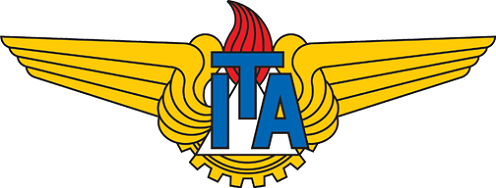
\includegraphics[height=0.65cm]{logos/ita}}

%---------------------------------------------------------------------
%  METADADOS
%---------------------------------------------------------------------
\title[Identificacao de Drone VTOL]{Identificação de Modelo Matemático de\\ Drone VTOL em modo multirrotor}
\author[H.\,M.\,S. Corrêa]{Henrique Mark dos Santos Corrêa}
\institute[ITA]{Programa de Pós-Graduação em Engenharia Aeronáutica e Mecânica\\
                Instituto Tecnológico de Aeronáutica --- ITA}
\date{Defesa de Mestrado \\ São José dos Campos, 2026}  % <-- ajuste a data

\newcommand{\orientadora}{Prof.\textsuperscript{a}~Dr.\textsuperscript{a}~Neusa Maria Franco de Oliveira}

%---------------------------------------------------------------------
%  Sumario no inicio de cada secao
%---------------------------------------------------------------------
\AtBeginSection[]{%
  \begin{frame}{Sumário}
    \tableofcontents[currentsection]
  \end{frame}}

\begin{document}

%=====================================================================
%  CAPA
%=====================================================================
\begin{frame}[plain]
  % >>> LOGO DO ITA na capa (arquivo: logos/ita.jpg). Troque por um oficial se quiser.
  \begin{center}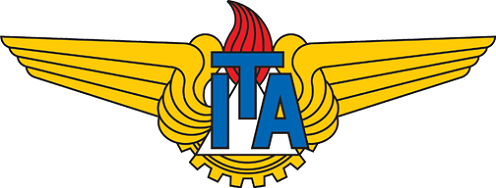
\includegraphics[height=1.5cm]{logos/ita}\end{center}
  \titlepage
  \begin{center}
    \small Orientadora: \orientadora
  \end{center}
\end{frame}

%=====================================================================
%  SUMARIO
%=====================================================================
\begin{frame}{Sumário}
  \tableofcontents
\end{frame}

%=====================================================================
\section{Introdução}
%=====================================================================
\begin{frame}{Contexto: VANTs de asa fixa e multirrotor}
  Os \textbf{VANTs} (Veículos Aéreos Não Tripulados), aeronaves que operam sem piloto a bordo, de forma remota ou autônoma, vêm ganhando destaque em áreas como vigilância, agricultura e georreferenciamento~\cite{Shakhatreh2019}. Esse avanço é impulsionado por microcontroladores mais rápidos e sensores mais precisos, que viabilizam algoritmos de controle mais sofisticados e, portanto, maior autonomia e segurança nas aplicações~\cite{Hassanalian2017}.
  \vfill
  \begin{columns}[T]
    \begin{column}{0.48\textwidth}
      \begin{block}{Multirrotor (asa rotativa)}
        Alta manobrabilidade, estabilidade e precisão espacial; \\[0.3em]
        porém \textbf{baixa autonomia} energética.
      \end{block}
    \end{column}
    \begin{column}{0.48\textwidth}
      \begin{block}{Asa fixa}
        Alta eficiência e autonomia (longas distâncias); \\[0.3em]
        porém \textbf{exige pista} para decolar e pousar.
      \end{block}
    \end{column}
  \end{columns}
  \vfill
  As limitações de cada tipo motivam uma solução intermediária: o VTOL~\cite{Brito2019}.
\end{frame}

\begin{frame}{VTOL: unindo os dois mundos}
  \begin{itemize}
    \item Decola e pousa na vertical (modo multirrotor) e percorre longas distâncias com eficiência energética (modo asa fixa)~\cite{Saeed2018}.
  \end{itemize}
  \vfill
  \begin{columns}[b]
    \begin{column}{0.32\textwidth}\centering
      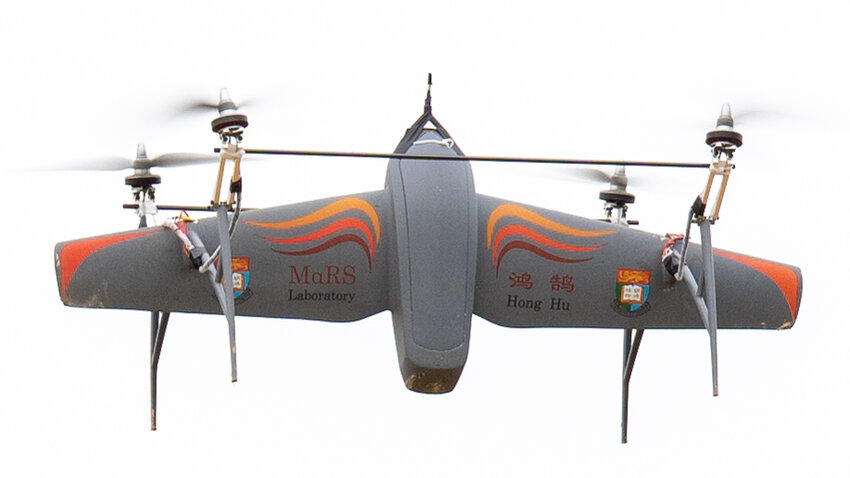
\includegraphics[height=2.7cm]{figuras/VTOL-TAIL}\\[0.3em]\small (a) Tailsitter
    \end{column}
    \begin{column}{0.32\textwidth}\centering
      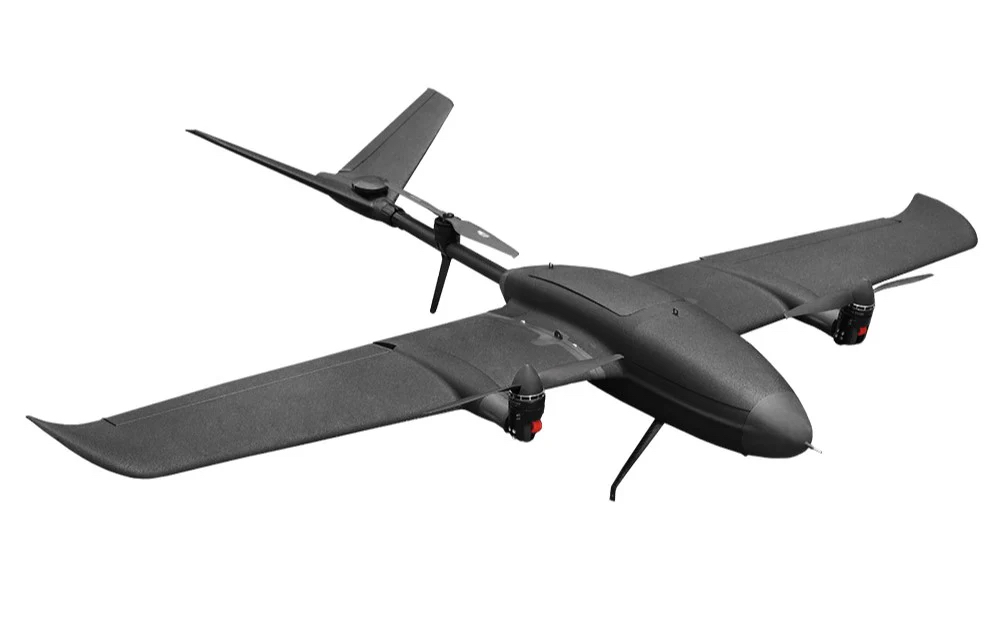
\includegraphics[height=2.7cm]{figuras/VTOL-TILT}\\[0.3em]\small (b) Tiltrotor
    \end{column}
    \begin{column}{0.32\textwidth}\centering
      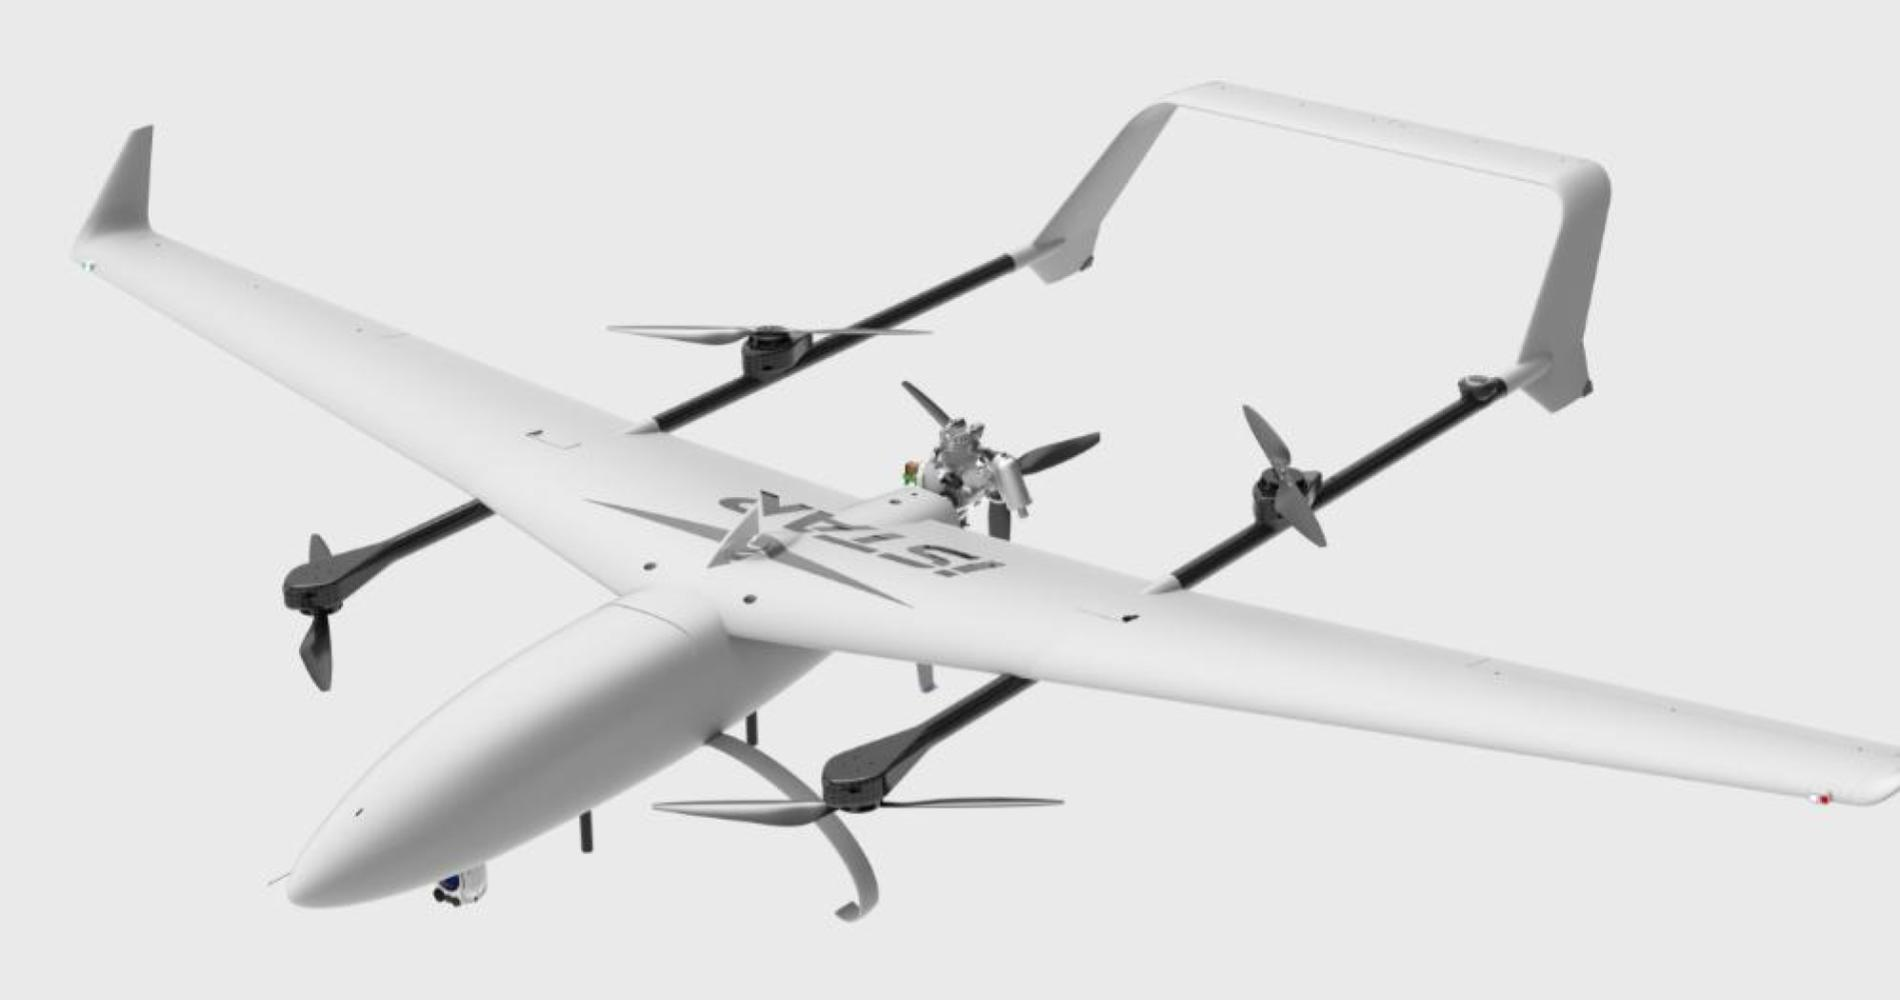
\includegraphics[height=2.7cm]{figuras/VTOL}\\[0.3em]\small \textbf{\color{itaAzul}(c) Híbrida} — foco
    \end{column}
  \end{columns}
  \vfill
  \footnotesize A configuração híbrida mantém a orientação do motor e simplifica a transição~\cite{Graesdal2021}.
\end{frame}

\begin{frame}{O Drone Híbrido e o desafio de modelar}
  \begin{columns}[c]
    \begin{column}{0.40\textwidth}\centering
      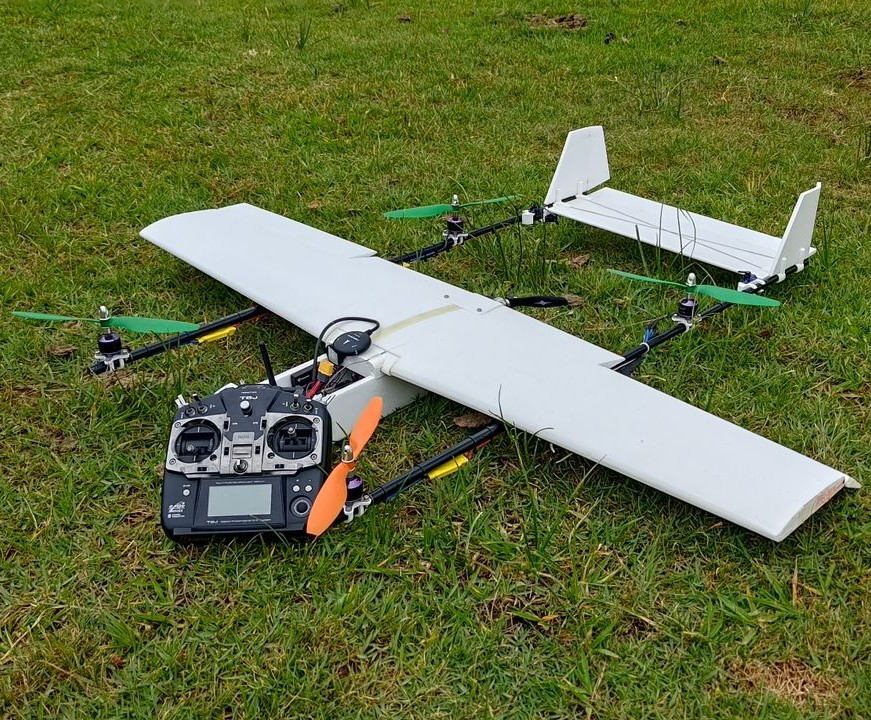
\includegraphics[width=\linewidth]{figuras/DH-REAL}\\[0.3em]{\footnotesize Drone Híbrido (DH). Fonte: De Lucena et al. (2025)}
    \end{column}
    \begin{column}{0.60\textwidth}
      \begin{itemize}
        \item Une os efeitos do modo multirrotor e da aerodinâmica de asa fixa, elevando a complexidade do modelo~\cite{Graesdal2021}.
        \item O modo multirrotor é \alert{instável}: não se excita em malha aberta~\cite{Aguirre2015}.
        \item Modelo apenas por geometria/bancada não garante fidelidade (inércias, constantes dos motores, dinâmicas não modeladas).
      \end{itemize}
    \end{column}
  \end{columns}
\end{frame}

\begin{frame}{Motivação}
  \begin{itemize}
    \item Projetar controle exige um \textbf{modelo dinâmico representativo} da aeronave.
    \item Obtê-lo é custoso e incerto: sintonia empírica de ganhos, campanhas de voo extensas, risco de acidentes.
    \item Modelos genéricos ou apenas de bancada não representam fielmente o VTOL híbrido.
  \end{itemize}
  \vfill
  \begin{block}{Motivação central}
    Obter um modelo \textbf{representativo e validado} do VTOL em modo multirrotor por meio de \textbf{identificação de sistemas a partir de dados reais de voo}~\cite{Jategaonkar2015, Aguirre2015}.
  \end{block}
\end{frame}

\begin{frame}{Objetivos}
  \begin{block}{Objetivo geral}
    Identificar e validar um modelo matemático do drone VTOL híbrido em modo multirrotor, a partir de dados de voo (treino e validação), apoiando o projeto de controle de decolagem.
  \end{block}
  \textbf{Objetivos específicos:}
  \begin{enumerate}
    \item Modelagem matemática em modo quadricóptero: modelo não-linear e aproximação linear.
    \item Projeto de manobras e coleta dos dados de voo.
    \item Identificação do modelo a partir dos dados (OEM / metodologia M4V)~\cite{Jategaonkar2015}.
    \item Validação do modelo identificado.
    \item Projeto e simulação do controle (PID em cascata), comparando a resposta nos modelos linear e não-linear.
  \end{enumerate}
\end{frame}

%=====================================================================
\section{Modelagem Matemática}
%=====================================================================
\begin{frame}{Referencial de navegação}
  \begin{columns}[c]
    \begin{column}{0.52\textwidth}\centering
      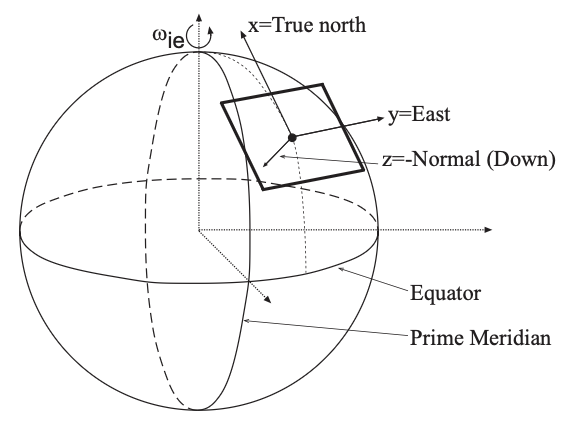
\includegraphics[width=\linewidth]{figuras/NAVIGATION-FRAME}\\[0.3em]{\footnotesize Plano tangente local (NED). Fonte: Farrell (2008)}
    \end{column}
    \begin{column}{0.48\textwidth}
      \begin{itemize}
        \item A Terra é aproximada por um \textbf{plano tangente} local (aeronave de pequeno porte)~\cite{Farrell2008}.
        \item Referencial de navegação $\mathcal{F}^{g}$, fixo à superfície.
        \item Posição em \textbf{NED}: $\mathbf{p}^{g}=[x,y,h]^{\top}$ \\ (norte $x$, leste $y$, altitude $h$).
      \end{itemize}
    \end{column}
  \end{columns}
\end{frame}

\begin{frame}{Referencial do corpo e atitude}
  \begin{columns}[c]
    \begin{column}{0.52\textwidth}\centering
      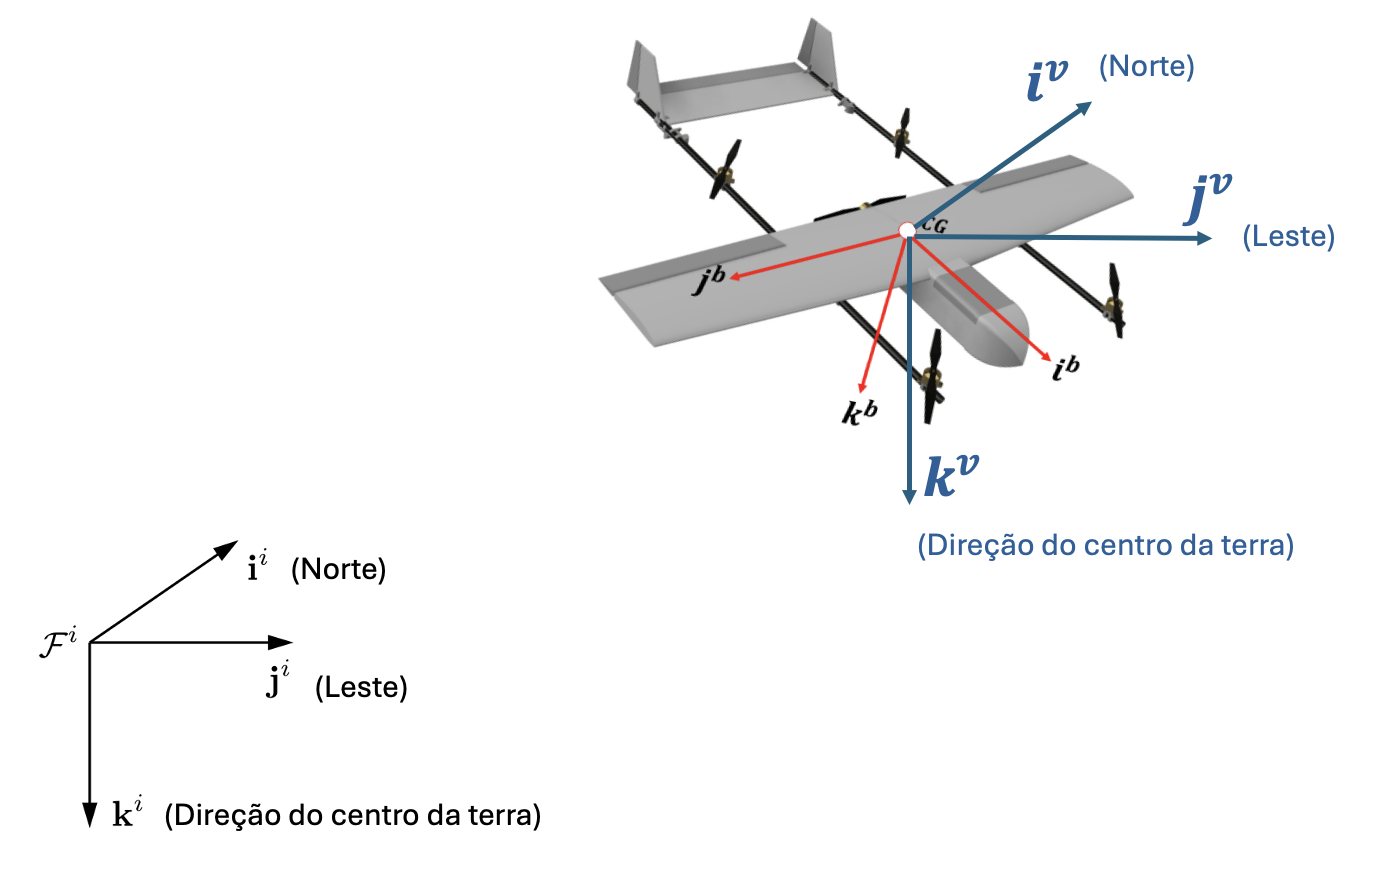
\includegraphics[width=\linewidth]{figuras/NAV}\\[0.3em]{\footnotesize Referenciais de navegação e do corpo. Fonte: adaptado de Beard e McLain (2012)}
    \end{column}
    \begin{column}{0.48\textwidth}
      \begin{itemize}
        \item Referencial do corpo $\mathcal{F}^{b}$, fixo ao CG: eixos $i^{b}$ (frente), $j^{b}$ (direita), $k^{b}$ (baixo).
        \item Velocidade linear do corpo: $\mathbf{v}_b=[u,v,w]^{\top}$.
        \item Velocidade angular do corpo: $\boldsymbol{\omega}_b=[p,q,r]^{\top}$.
        \item Atitude por ângulos de Euler: rolagem $\phi$, arfagem $\theta$, guinada $\psi$.
      \end{itemize}
    \end{column}
  \end{columns}
\end{frame}

\begin{frame}{Transformação de coordenadas}
  Três rotações elementares (guinada, arfagem, rolagem) compõem a matriz corpo~$\to$~navegação~\cite{Farrell2008}:
  \begin{equation}
    \mathbf{R}^{g}_{b} = \mathbf{R}_z(\psi)\,\mathbf{R}_y(\theta)\,\mathbf{R}_x(\phi)
    = {\scriptsize\begin{bmatrix}
      c_\theta c_\psi & s_\phi s_\theta c_\psi - c_\phi s_\psi & c_\phi s_\theta c_\psi + s_\phi s_\psi \\[2pt]
      c_\theta s_\psi & s_\phi s_\theta s_\psi + c_\phi c_\psi & c_\phi s_\theta s_\psi - s_\phi c_\psi \\[2pt]
      -s_\theta & s_\phi c_\theta & c_\phi c_\theta
    \end{bmatrix}} \tag{2.3}
  \end{equation}
  Ortonormal: $\mathbf{R}^{b}_{g} = (\mathbf{R}^{g}_{b})^{\top}$. Projetando a gravidade no corpo (usada adiante):
  \begin{equation}
    \mathbf{g}^{b} = (\mathbf{R}^{g}_{b})^{\top}\!\begin{bmatrix}0\\0\\g\end{bmatrix}
    = \begin{bmatrix} -g\,s_\theta \\ g\,s_\phi c_\theta \\ g\,c_\phi c_\theta \end{bmatrix} \tag{2.5}
  \end{equation}
  \vfill
  {\footnotesize Notação: $c_\ast=\cos(\ast)$, $s_\ast=\sin(\ast)$, $t_\ast=\tan(\ast)$.}
\end{frame}

%=====================================================================
\begin{frame}{Estrutura do modelo não-linear}
  Com os referenciais estabelecidos, o modelo não-linear do modo quadricóptero relaciona o comando dos motores às saídas do corpo rígido ($\dot{x}=f(x,u,\Theta)$). As próximas seções detalham cada bloco:
  \begin{center}
    \resizebox{!}{5.4cm}{%
    \begin{tikzpicture}[
        sysblock/.style={rectangle, draw=blkEdge, semithick, fill=blkBase, rounded corners=3pt, minimum height=1.4cm, text width=2.2cm, align=center, font=\footnotesize},
        hi/.style={fill=blkHi, draw=blkHiEdge, thick},
        io/.style={font=\footnotesize},
        arr/.style={-{Stealth[length=2.5mm]}, semithick, black!62},
        darr/.style={-{Stealth[length=2.5mm]}, semithick, black!48, dashed},
        lbl/.style={font=\scriptsize, fill=white, inner sep=1.5pt, text=black!80},
        dot/.style={circle, fill=black!62, inner sep=0pt, minimum size=4pt},
    ]
    \node[io, align=center] at (0,0) (sig) {$\sigma_i$\\(PWM)};
    \node[sysblock, hi, text width=1.9cm] at (2.7,0) (motor) {Modelo do\\Motor};
    \node[sysblock, text width=1.8cm] at (5.5,0) (balloc) {Matriz de\\alocação $\mathbf{B}$};
    \node[sysblock, hi] at (8.3,0) (rotdyn) {Dinâmica\\Rotacional\\$\dot{p},\dot{q},\dot{r}$};
    \draw[arr] (sig) -- (motor);
    \draw[arr] ([yshift=0.22cm]motor.east) -- node[lbl, above] {$T_i$} ([yshift=0.22cm]balloc.west);
    \draw[arr] ([yshift=-0.22cm]motor.east) -- node[lbl, below] {$Q_i$} ([yshift=-0.22cm]balloc.west);
    \draw[arr] (balloc) -- node[lbl, above] {$\tau_x,\tau_y,\tau_z$} (rotdyn);
    \node[io] at (10.6,0) (pqr_out) {$p, q, r$};
    \draw[arr] (rotdyn) -- (pqr_out);
    \node[sysblock] at (8.3,-4) (euler) {Cinemática\\de Euler\\$\dot{\phi},\dot{\theta},\dot{\psi}$};
    \node[io] at (10.6,-4) (att_out) {$\phi, \theta, \psi$};
    \draw[arr] (euler) -- (att_out);
    \node[sysblock, hi] at (8.3,-8) (transdyn) {Dinâmica\\Translacional\\$\dot{u},\dot{v},\dot{w}$};
    \node[io] at (10.6,-7.7) (uvw_out) {$u, v, w$};
    \node[io] at (10.6,-8.3) (acc_out) {$\dot{u}, \dot{v}, \dot{w}$};
    \draw[arr] ([yshift=0.3cm]transdyn.east) -- (uvw_out);
    \draw[arr] ([yshift=-0.3cm]transdyn.east) -- (acc_out);
    \node[io] at (6.1,-8.35) (const) {$m, g$};
    \draw[arr] (const) -- ([yshift=-0.35cm]transdyn.west);
    \draw[arr] (balloc.south) -- (5.5,-8.0) -- node[lbl, above] {$T$} ([yshift=0.0cm]transdyn.west);
    \node[dot] at (8.3,-1.5) (junc) {};
    \draw[semithick, black!62] (rotdyn.south) -- (junc);
    \draw[arr] (junc) -- node[lbl, left] {$p,q,r$} (euler.north);
    \draw[darr] (junc.west) -- (6.9,-1.5) -- (6.9,-7.65) -- ([yshift=0.35cm]transdyn.west);
    \draw[arr] (euler.south) -- node[lbl, left] {$\phi,\theta,\psi$} (transdyn.north);
    \end{tikzpicture}}
  \end{center}
\end{frame}

\begin{frame}{Modelo de propulsão do motor}
  Estrutura em dois estágios~\cite{Quan2017}: o comando PWM é normalizado e define a velocidade do rotor (regime permanente e atraso de 1ª ordem).
  \begin{center}
    
\includegraphics[width=0.68\linewidth]{figuras/blocos-motor}\\[0.2em]
    {\footnotesize Modelo do motor em dois estágios. Fonte: adaptado de Quan (2017).}
  \end{center}
  \small
  \begin{columns}[T]
    \begin{column}{0.5\textwidth}
      \centering\textbf{Normalização do PWM}
      \[ \sigma_i = \frac{\delta_{PWM,i}-\delta_{\min}}{\delta_{\max}-\delta_{\min}} \in [0,1] \]
      {\footnotesize $\delta_{\min}=1000\,\mu$s,\; $\delta_{\max}=2000\,\mu$s}
    \end{column}
    \begin{column}{0.5\textwidth}
      \centering\textbf{Velocidade do rotor}
      \begin{align*}
        \Omega_{ss,i} &= C_R\,\sigma_i + \Omega_b \tag{2.6}\\
        \Omega_i &= \tfrac{1}{\tau_m s + 1}\,\Omega_{ss,i} \tag{2.7}
      \end{align*}
    \end{column}
  \end{columns}
\end{frame}

\begin{frame}{Empuxo e torque do rotor}
  Cada rotor, girando a $\Omega_i$, produz um empuxo e um torque de reação proporcionais ao quadrado da velocidade angular~\cite{Graesdal2021,Quan2017}:
  \begin{align*}
    T_i &= c_{T_i}\,\Omega_i^{2} \tag{2.8}\\[0.3em]
    Q_i &= c_{M_i}\,\Omega_i^{2} \tag{2.9}
  \end{align*}
  \vfill
  \begin{itemize}
    \item $c_{T_i},\,c_{M_i}$: coeficientes de empuxo e de torque de cada motor.
    \item Dependem da geometria da hélice e da densidade do ar; obtidos em \textbf{ensaios de bancada} (Apêndice).
    \item A razão $c_M/c_T$ define a contribuição de guinada na matriz de alocação.
  \end{itemize}
\end{frame}

\begin{frame}{Alocação dos motores}
  A matriz de alocação $\mathbf{B}$ combina os empuxos individuais $T_i$ no empuxo total $T$ e nos momentos de controle $\tau_x,\tau_y,\tau_z$ (função da geometria e da razão $c_M/c_T$):
  \vfill
  \begin{equation}
    \begin{bmatrix} T \\ \tau_x \\ \tau_y \\ \tau_z \end{bmatrix} =
    \begin{bmatrix}
      1 & 1 & 1 & 1 \\
      -L_{x_r} & L_{x_l} & L_{x_l} & -L_{x_r} \\
      L_{y_f} & -L_{y_r} & L_{y_f} & -L_{y_r} \\
      \tfrac{c_M}{c_T} & \tfrac{c_M}{c_T} & -\tfrac{c_M}{c_T} & -\tfrac{c_M}{c_T}
    \end{bmatrix}
    \begin{bmatrix} T_1 \\ T_2 \\ T_3 \\ T_4 \end{bmatrix}
    \tag{2.15}
  \end{equation}
\end{frame}

\begin{frame}{Modelo rotacional: dedução}
  \textbf{2ª lei de Newton} para a rotação ($\mathbf{h}$: momento angular; $\boldsymbol\tau$: soma dos momentos aplicados)~\cite{Beard2012}:
  \begin{equation}\frac{d\mathbf{h}}{dt}=\boldsymbol\tau\tag{2.16}\end{equation}
  Transportando para o corpo, com $\mathbf{h}^{b}=\mathbf{J}\,\boldsymbol\omega_b$ e $\boldsymbol\tau^{b}=[\tau_x,\tau_y,\tau_z]^{\top}$ (momentos de controle dos motores, via matriz $\mathbf{B}$):
  \begin{equation}\frac{d\mathbf{h}^{b}}{dt}+\boldsymbol\omega_b\times\mathbf{h}^{b}=\boldsymbol\tau^{b}\tag{2.17}\end{equation}
  Tensor de inércia \alert{não-diagonal} ($J_{xz}\neq 0$, pela estrutura de asa fixa), resultando na dinâmica rotacional:
  \begin{equation}
    \mathbf{J}=\begin{bmatrix} J_{xx} & 0 & -J_{xz} \\ 0 & J_{yy} & 0 \\ -J_{xz} & 0 & J_{zz} \end{bmatrix}
    \;\Rightarrow\;
    \dot{\boldsymbol\omega}_b=\mathbf{J}^{-1}\!\left[-\boldsymbol\omega_b\times(\mathbf{J}\boldsymbol\omega_b)+\boldsymbol\tau^{b}\right]
    \tag{2.20}
  \end{equation}
\end{frame}

\begin{frame}{Modelo rotacional: forma final}
  Incluindo o \textbf{arrasto angular} ($c_p,c_q,c_r$, proporcional a $p,q,r$)~\cite{Quan2017} e reduzindo ao modo quadricóptero (arrasto de asa fixa desprezível):
  \begin{align*}
    \dot{p} &= \Gamma_1\,pq - \Gamma_2\,qr + \Gamma_3\,\tau_x + \Gamma_4\,\tau_z - c_p\,p \tag{2.22}\\
    \dot{q} &= \Gamma_5\,pr - \Gamma_6\,(p^2 - r^2) + \tfrac{1}{J_y}\,\tau_y - c_q\,q \tag{2.23}\\
    \dot{r} &= \Gamma_7\,pq - \Gamma_1\,qr + \Gamma_4\,\tau_x + \Gamma_8\,\tau_z - c_r\,r \tag{2.24}
  \end{align*}
  \footnotesize com $\Gamma = J_x J_z - J_{xz}^{2}$ e:
  \[
    \begin{array}{llll}
      \Gamma_1=\tfrac{J_{xz}(J_x-J_y+J_z)}{\Gamma} &
      \Gamma_2=\tfrac{J_z(J_z-J_y)+J_{xz}^2}{\Gamma} &
      \Gamma_3=\tfrac{J_z}{\Gamma} &
      \Gamma_4=\tfrac{J_{xz}}{\Gamma} \\[4pt]
      \Gamma_5=\tfrac{J_z-J_x}{J_y} &
      \Gamma_6=\tfrac{J_{xz}}{J_y} &
      \Gamma_7=\tfrac{(J_x-J_y)J_x+J_{xz}^2}{\Gamma} &
      \Gamma_8=\tfrac{J_x}{\Gamma}
    \end{array}
  \]
\end{frame}

\begin{frame}{Modelo translacional: dedução}
  \textbf{2ª lei de Newton} para a translação~\cite{Beard2012,Graesdal2021}:
  \begin{equation}m\frac{d\mathbf{v}}{dt}=\mathbf{f}\tag{2.25}\end{equation}
  Transportando para o referencial do corpo, com $\dot{\mathbf{v}}=[\dot u,\dot v,\dot w]^{\top}$:
  \begin{equation}m\big(\dot{\mathbf{v}}+\boldsymbol\omega_b\times\mathbf{v}\big)=\mathbf{f}\tag{2.26}\end{equation}
  As forças são o empuxo (propulsão) e a gravidade projetada no corpo, $\mathbf{f}=\mathbf{f}_{\text{prop}}+\mathbf{f}_{g}$:
  \begin{equation} \mathbf{f}_{\text{prop}}=\begin{bmatrix}0\\0\\-T\end{bmatrix}, \qquad
     \mathbf{f}_{g}=m\,\mathbf{g}^{b}=mg\begin{bmatrix}-s_\theta\\ s_\phi c_\theta\\ c_\phi c_\theta\end{bmatrix} \tag{2.27}\end{equation}
\end{frame}

\begin{frame}{Modelo translacional: forma final}
  Dividindo por $m$ e assumindo velocidade longitudinal desprezível (sem sustentação/arrasto de asa fixa), obtêm-se as equações do modelo translacional:
  \begin{align*}
    \dot{u} &= rv - qw - g\,s_\theta \tag{2.29}\\
    \dot{v} &= pw - ru + g\,s_\phi c_\theta \tag{2.30}\\
    \dot{w} &= qu - pv - \tfrac{T}{m} + g\,c_\phi c_\theta \tag{2.31}
  \end{align*}
\end{frame}

\begin{frame}{Saída do acelerômetro (IMU)}
  \begin{columns}[c]
    \begin{column}{0.34\textwidth}\centering
      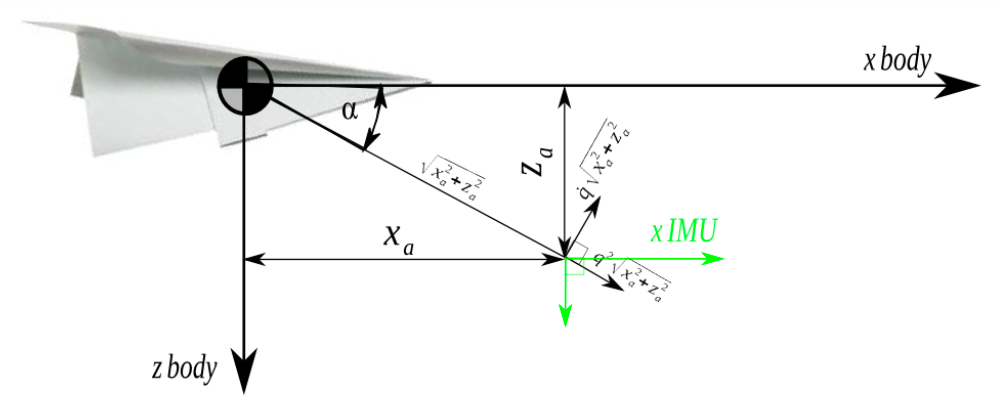
\includegraphics[width=\linewidth]{figuras/ACELEROMETER}\\[0.2em]{\footnotesize IMU deslocada do CG por $\mathbf{r}_{imu}$ (Fig.~2.9)}
    \end{column}
    \begin{column}{0.66\textwidth}
      A IMU mede a força específica no ponto de montagem; do CG somam-se termos tangencial e centrípeto~\cite{Tischler2012}:
      \begin{equation}
        \mathbf{a}_{imu}^{b}=\mathbf{a}_{cg}^{b}
        + \dot{\boldsymbol\omega}^{b}\times\mathbf{r}_{imu}
        + \boldsymbol\omega^{b}\times(\boldsymbol\omega^{b}\times\mathbf{r}_{imu})
        + \mathbf{b}
        \tag{2.32}
      \end{equation}
      \scriptsize
      \begin{align*}
        a_x &= (\dot q\,r_z - \dot r\,r_y) + pq\,r_y + pr\,r_z - (q^2+r^2)r_x + b_x \tag{2.33}\\        a_y &= (\dot r\,r_x - \dot p\,r_z) + pq\,r_x + qr\,r_z - (p^2+r^2)r_y + b_y \tag{2.34}\\        a_z &= -\tfrac{T}{m} + (\dot p\,r_y - \dot q\,r_x) + pr\,r_x + qr\,r_y - (p^2+q^2)r_z + b_z \tag{2.35}      \end{align*}
    \end{column}
  \end{columns}
  \vfill
  {\footnotesize O deslocamento acopla $\dot p,\dot q,\dot r$ e $p,q,r$ à medida $\Rightarrow$ informação útil para a identificação.}
\end{frame}

\begin{frame}{Cinemática de Euler}
  Relação entre as velocidades angulares do corpo e as taxas dos ângulos de Euler~\cite{Farrell2008}:
  \begin{equation}
    \begin{bmatrix}\dot\phi\\\dot\theta\\\dot\psi\end{bmatrix}
    =\begin{bmatrix}
      1 & s_\phi\,t_\theta & c_\phi\,t_\theta \\[2pt]
      0 & c_\phi & -s_\phi \\[2pt]
      0 & s_\phi/c_\theta & c_\phi/c_\theta
    \end{bmatrix}
    \begin{bmatrix}p\\q\\r\end{bmatrix}
    \tag{2.36}
  \end{equation}
  \vfill
  \alert{Singularidade} em $\theta=\pm 90^\circ$ ($c_\theta=0$), fora do envelope de voo em modo multirrotor.
\end{frame}

\begin{frame}{Modelo não-linear completo (9 estados)}
  \small
  \begin{columns}[T]
    \begin{column}{0.5\textwidth}
      \textbf{Cinemática de atitude}
      \begin{align*}
        \dot\phi &= p + s_\phi t_\theta\,q + c_\phi t_\theta\,r \\
        \dot\theta &= c_\phi\,q - s_\phi\,r \\
        \dot\psi &= \tfrac{s_\phi}{c_\theta}\,q + \tfrac{c_\phi}{c_\theta}\,r
      \end{align*}
      \textbf{Dinâmica translacional}
      \begin{align*}
        \dot u &= rv - qw - g\,s_\theta \\
        \dot v &= pw - ru + g\,s_\phi c_\theta \\
        \dot w &= qu - pv - \tfrac{T}{m} + g\,c_\phi c_\theta
      \end{align*}
    \end{column}
    \begin{column}{0.5\textwidth}
      \textbf{Dinâmica rotacional}
      \begin{align*}
        \dot p &= \Gamma_1 pq - \Gamma_2 qr + \Gamma_3\tau_x + \Gamma_4\tau_z - c_p p \\
        \dot q &= \Gamma_5 pr - \Gamma_6(p^2-r^2) + \tfrac{1}{J_y}\tau_y - c_q q \\
        \dot r &= \Gamma_7 pq - \Gamma_1 qr + \Gamma_4\tau_x + \Gamma_8\tau_z - c_r r
      \end{align*}
      \vfill
      \begin{block}{}
        \centering $\dot{x}=f(x,u,\Theta)$ --- base para a identificação.
      \end{block}
    \end{column}
  \end{columns}
\end{frame}

%=====================================================================
\section{Plataforma e Instrumentação}
%=====================================================================
\begin{frame}{Plataforma: o Drone Híbrido (DH)}
  Protótipo VTOL híbrido, projetado e construído pela equipe~\cite{DeLucena2025}: \textbf{asa fixa} com motor \textit{pusher} de cauda (cruzeiro) ou \textbf{4 rotores em configuração H-Frame} (decolagem e pouso verticais). Este trabalho foca o \textbf{modo multirrotor}, em torno do voo pairado.
  \begin{center}
    
\includegraphics[width=0.82\linewidth]{figuras/drone}\\[0.2em]{\footnotesize Aeronave DH (Fig.~3.1)}
  \end{center}
  \vfill
  {\footnotesize Massa $1{,}993$~kg \;\textbar\; comprimento $1{,}05$~m \;\textbar\; envergadura $1{,}20$~m \;\textbar\; perfil USA-35B \;\textbar\; 4 motores SunnySky A2212 (1000~kV), hélices 10''.}
\end{frame}

\begin{frame}{Dimensões e matriz de alocação}
  \begin{columns}[c]
    \begin{column}{0.4\textwidth}\centering
      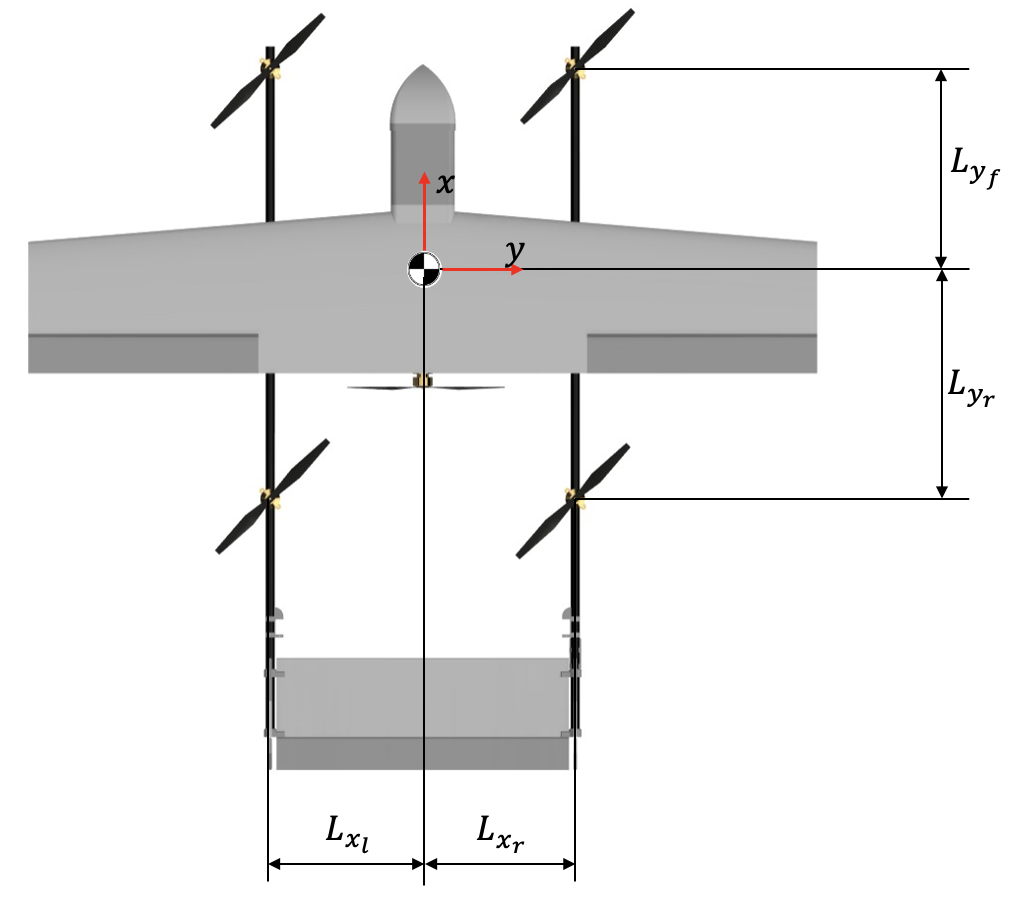
\includegraphics[width=\linewidth]{figuras/bracos}\\[0.2em]{\footnotesize Distâncias dos rotores ao CG (Fig.~3.2)}
    \end{column}
    \begin{column}{0.6\textwidth}
      \small
      Braços de momento medidos:
      \[ L_{x_l}=L_{x_r}=0{,}232~\text{m},\; L_{y_f}=0{,}330~\text{m},\; L_{y_r}=0{,}323~\text{m} \]
      Com $c_M/c_T=0{,}0286$~m (bancada), a alocação inicial:
      \begin{equation*} \mathbf{B}_0={\scriptsize\begin{bmatrix}
        1 & 1 & 1 & 1 \\
        -0{,}232 & 0{,}232 & 0{,}232 & -0{,}232 \\
        0{,}330 & -0{,}323 & 0{,}330 & -0{,}323 \\
        0{,}0286 & 0{,}0286 & -0{,}0286 & -0{,}0286
      \end{bmatrix}} \tag{3.1}\end{equation*}
    \end{column}
  \end{columns}
\end{frame}

\begin{frame}{Deslocamento do IMU}
  A IMU está deslocada do CG por $\mathbf{r}_{imu}$; esse braço de alavanca acopla as taxas angulares à leitura do acelerômetro (força específica), efeito modelado no Cap.~2.
  \begin{center}
    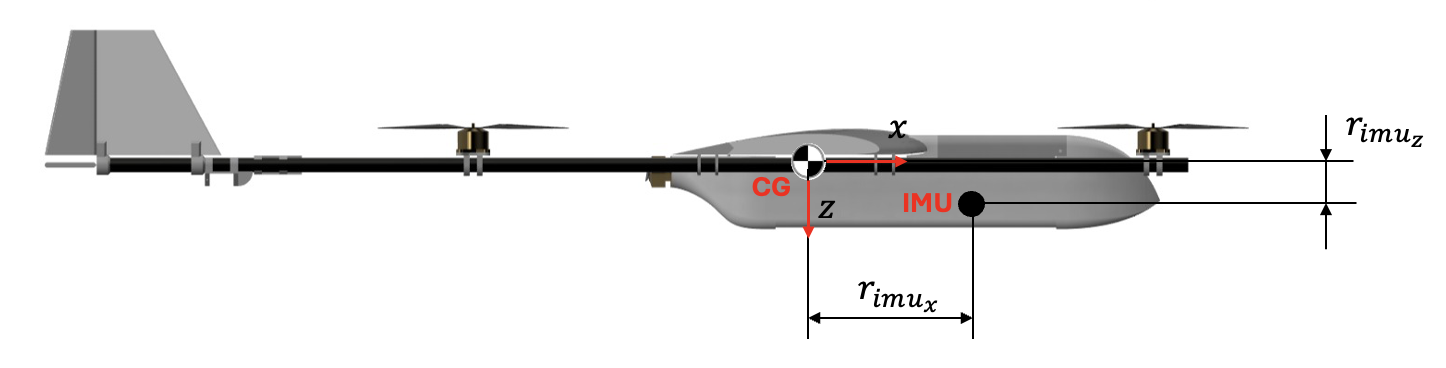
\includegraphics[width=0.92\linewidth]{figuras/displacement}
  \end{center}
  \vfill
  {\footnotesize Deslocamento medido da IMU em relação ao CG (Fig.~3.3); não pode ser desprezado na simulação da força específica.}
\end{frame}

\begin{frame}{Sistema de propulsão}
  \begin{columns}[c]
    \begin{column}{0.34\textwidth}\centering
      
\includegraphics[width=\linewidth]{figuras/motor}\\[0.2em]{\footnotesize Motopropulsor de sustentação (Fig.~3.4)}
    \end{column}
    \begin{column}{0.66\textwidth}
      \begin{itemize}
        \item \textbf{Motor:} 4 $\times$ SunnySky A2212 \textit{brushless}, 1000~kV, hélices de 10''.
        \item \textbf{ESC:} 30~A; converte o sinal de PWM (1000 a 2000~$\mu$s) no chaveamento trifásico do motor \textit{brushless}.
        \item $C_R,\Omega_b,c_T,c_M$ levantados em \textbf{ensaios de bancada}~\cite{Diorio2026}, que fornecem os valores iniciais do modelo do motor (Cap.~2).
      \end{itemize}
    \end{column}
  \end{columns}
\end{frame}

\begin{frame}{Aviônica e instrumentação}
  \begin{columns}[c]
    \begin{column}{0.3\textwidth}\centering
      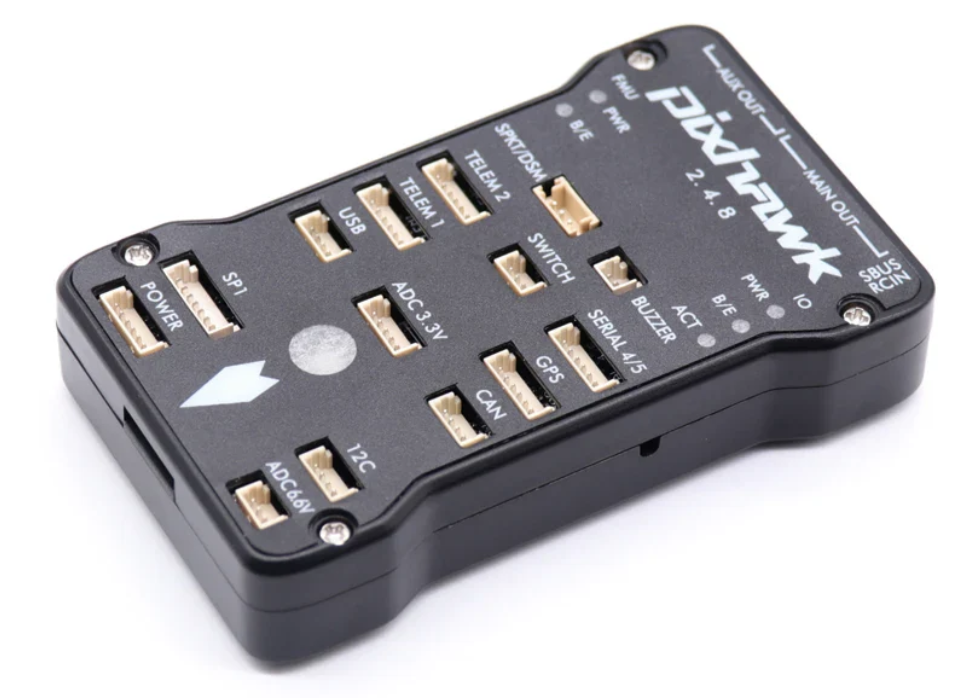
\includegraphics[width=\linewidth]{figuras/pixhawk}\\[0.2em]{\footnotesize Pixhawk 2.4.0 (Fig.~3.5)}
    \end{column}
    \begin{column}{0.7\textwidth}
      \begin{itemize}
        \item \textbf{Controladora:} Pixhawk 2.4.0~\cite{Cortez2022}, firmware ArduPilot; executa o controle e o EKF, e registra todos os dados de voo.
        \item \textbf{IMU} InvenSense MPU-6000: giroscópio $(p,q,r)$ e acelerômetro $(a_x,a_y,a_z)$, com taxa de amostragem de $25$~Hz.
        \item A atitude $(\phi,\theta,\psi)$ \alert{não é medida diretamente}: é estimada pelo EKF $\Rightarrow$ menor observabilidade da guinada.
      \end{itemize}
    \end{column}
  \end{columns}
\end{frame}

\begin{frame}{Campanha de voo}
  Série de manobras para excitar as principais dinâmicas do VTOL em modo multirrotor, realizada no ginásio do COCTA com a equipe do projeto Drone Híbrido.
  \begin{center}
    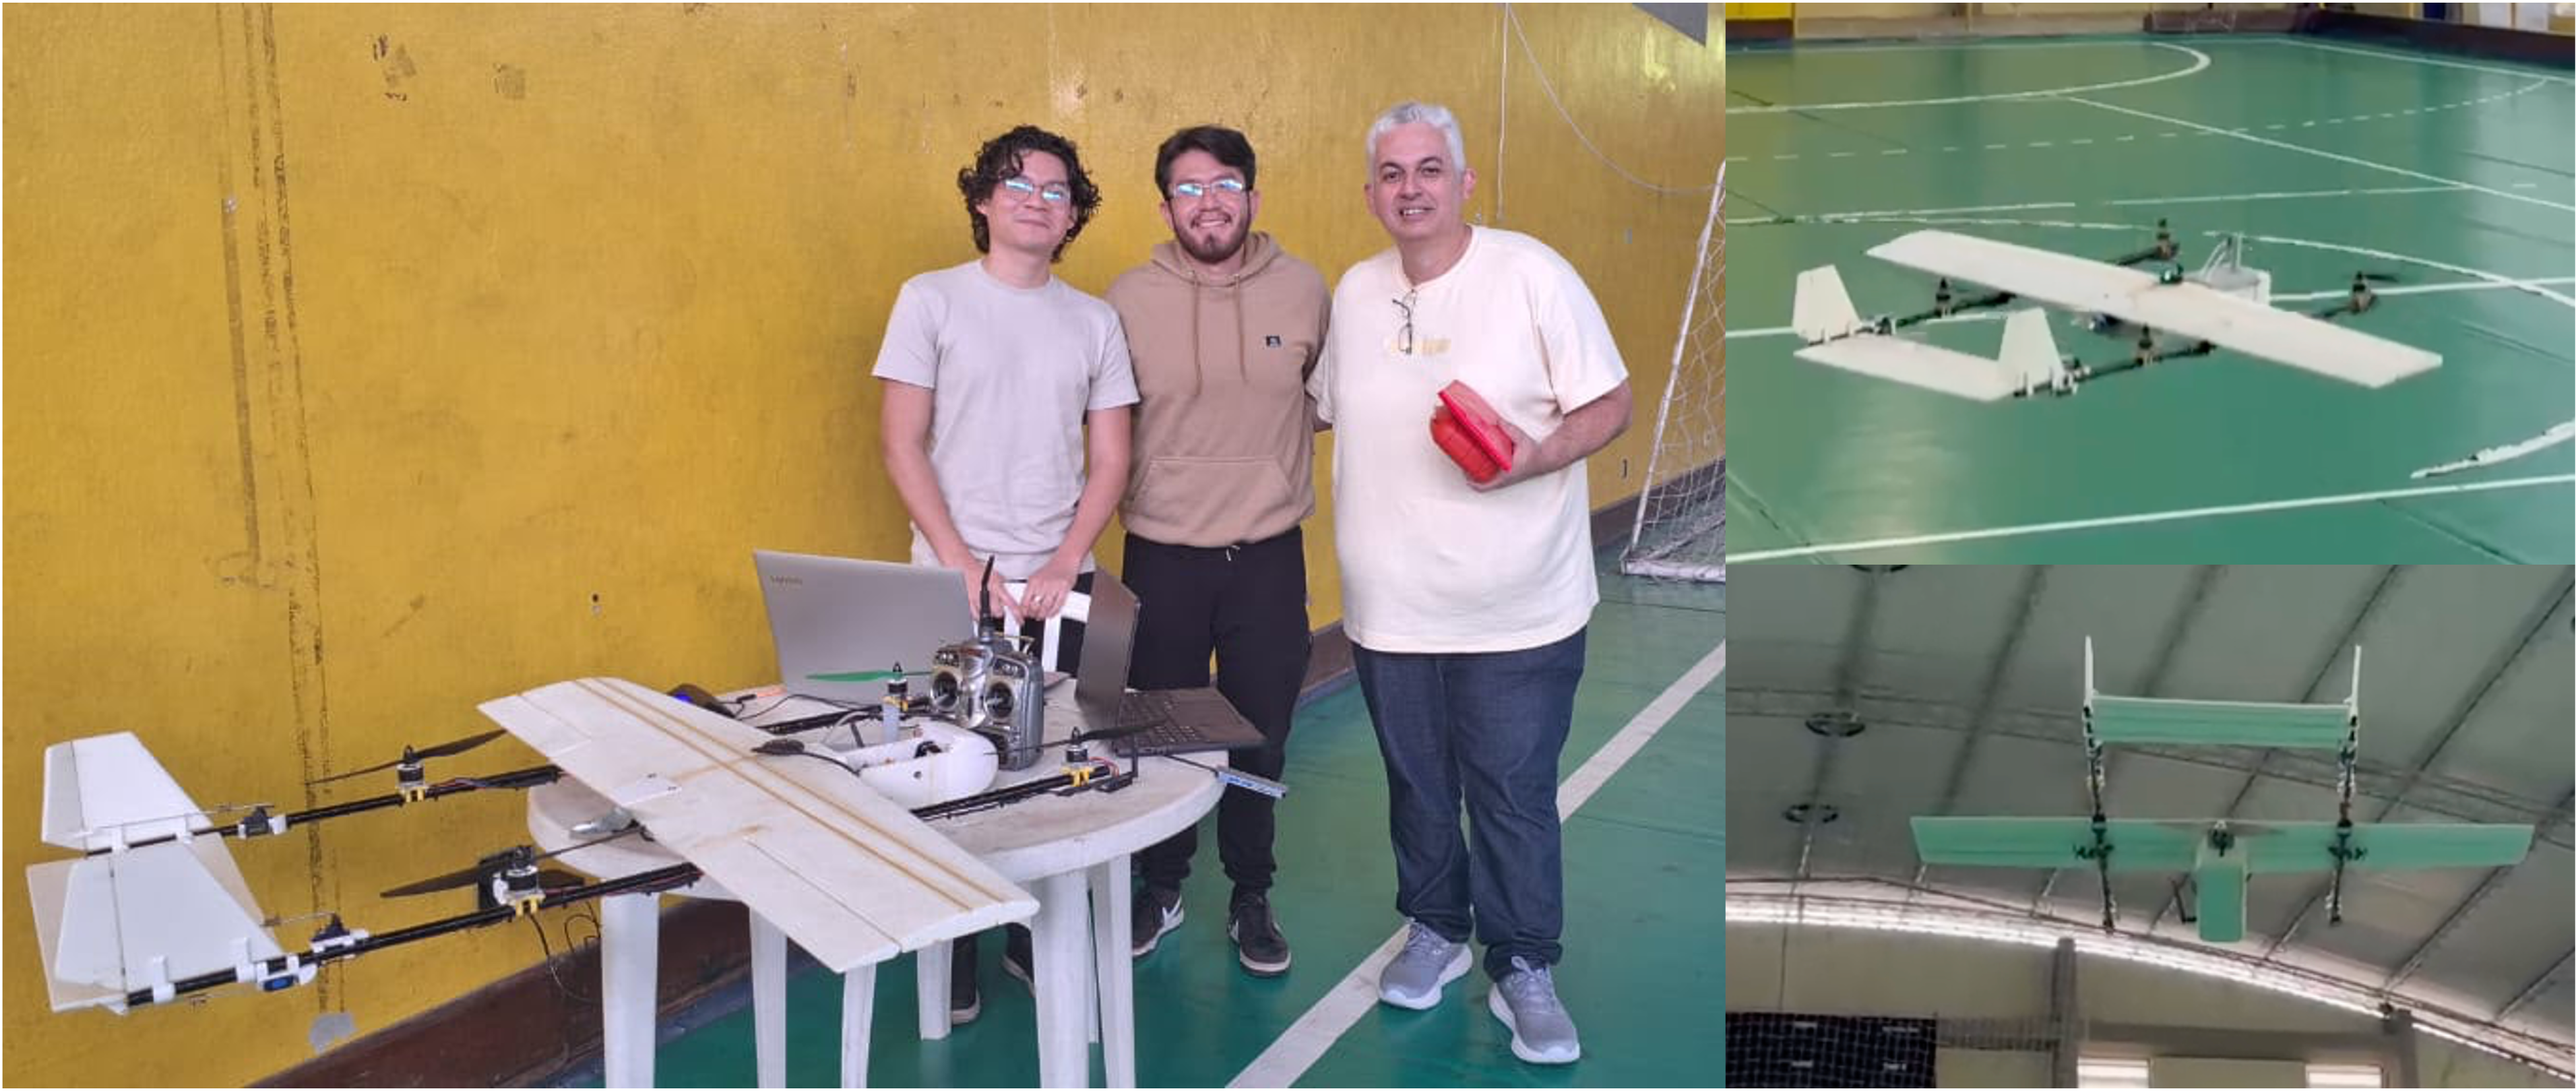
\includegraphics[width=0.66\linewidth]{figuras/voo1}\\[0.2em]
    {\footnotesize Campanha de voo no ginásio do COCTA (Fig.~3.6)}
  \end{center}
  {\footnotesize Trechos com quedas e perturbações foram descartados; selecionaram-se as melhores janelas para treino e validação.}
\end{frame}

\begin{frame}{Registro de voo: janelas de treino e validação}
  \begin{columns}[c]
    \begin{column}{0.62\textwidth}\centering
      
\includegraphics[width=\linewidth]{figuras/excitacao_dataset}\\[0.2em]
      {\footnotesize Campanha completa: RCIN, PWM, taxas e acelerações (Fig.~3.7)}
    \end{column}
    \begin{column}{0.38\textwidth}
      \textbf{Treino} (eixos isolados, verde):
      \begin{itemize}\footnotesize
        \item Guinada: $0$ a $40$~s
        \item Rolagem: $40$ a $80$~s
        \item Arfagem: $80$ a $125$~s
      \end{itemize}
      \textbf{Validação} (movimento composto, laranja):
      \begin{itemize}\footnotesize
        \item $450$ a $470$~s e $605$ a $625$~s
      \end{itemize}
      {\footnotesize Os três eixos excitados ao mesmo tempo, isolados dos dados de treino.}
    \end{column}
  \end{columns}
\end{frame}

%=====================================================================
\section{Metodologia de Identificação}
%=====================================================================
\begin{frame}{Sistemas instáveis: qual laço identificar?}
  O quadrirotor é \textbf{instável} em malha aberta e voa estabilizado por um controlador~\cite{Jategaonkar2015}.
  \begin{center}
    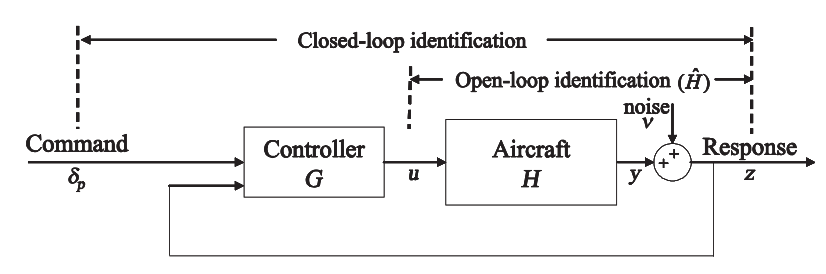
\includegraphics[width=0.8\linewidth]{figuras/identification}\\[0.2em]
    {\footnotesize Identificação de sistema instável com controlador. Fonte: adaptado de Jategaonkar (2015)}
  \end{center}
  \begin{itemize}
    \item \textbf{Malha fechada} ($\boldsymbol{\sigma_P}\!\to\!z$): reproduz comando e resposta, mas mistura planta e controlador.
    \item \textbf{Malha aberta na planta} ($u\!\to\!z$): estima os parâmetros físicos do VTOL. \alert{Adotada}, como em~\cite{Matt2025, Niermeyer2015}.
  \end{itemize}
\end{frame}

\begin{frame}{Método M4V}
  \begin{columns}[c]
    \begin{column}{0.46\textwidth}\centering
      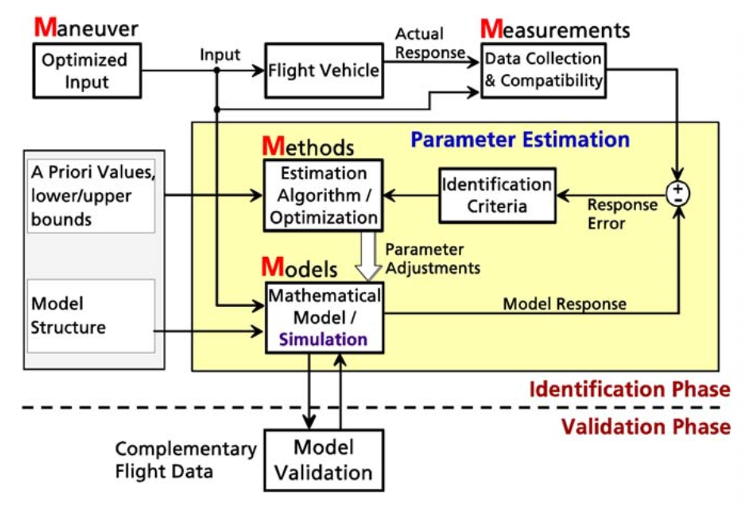
\includegraphics[width=\linewidth]{figuras/m4v}\\[0.2em]
      {\footnotesize Metodologia iterativa M4V. Fonte: adaptado de Jategaonkar (2015)}
    \end{column}
    \begin{column}{0.54\textwidth}
      Abordagem sistemática e iterativa no domínio do tempo, consolidada na identificação de aeronaves~\cite{Jategaonkar2015, Tischler2012}. Cinco etapas:
      \begin{enumerate}
        \item \textbf{Manobras} (\textit{Maneuvers})
        \item \textbf{Medições} (\textit{Measurements})
        \item \textbf{Métodos} (\textit{Methods})
        \item \textbf{Modelos} (\textit{Models})
        \item \textbf{Validação} (\textit{Validation})
      \end{enumerate}
    \end{column}
  \end{columns}
\end{frame}

\begin{frame}{Manobras: cadeia de excitação}
  A excitação não é aplicada à planta, mas somada à saída do controlador, um eixo de cada vez (\textit{separate surface excitation})~\cite{Jategaonkar2015}.
  \begin{center}
    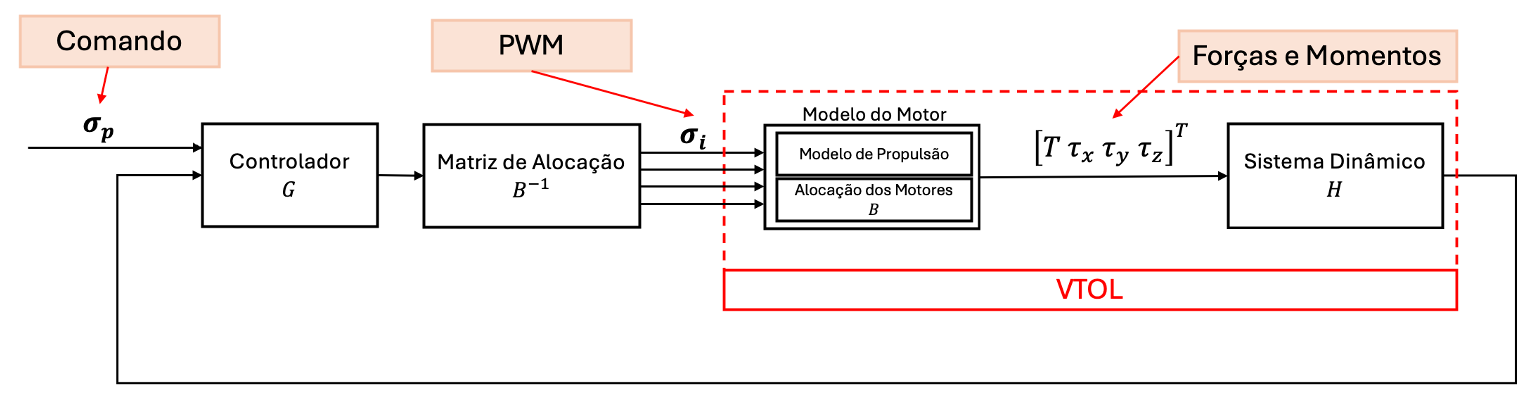
\includegraphics[width=\linewidth]{figuras/entradas}\\[0.2em]
    {\footnotesize Comando do piloto $\boldsymbol{\sigma_P}$ $\to$ controlador $+$ \textit{mixer} $\mathbf{B}^{-1}$ $\to$ PWM $\sigma_i$ $\to$ modelo do motor $\to$ momentos $\tau$ (Fig.~4.4)}
  \end{center}
  A entrada efetivamente analisada é o \textbf{momento $\tau$} do eixo excitado, e não o PWM bruto nem o comando do piloto.
\end{frame}

\begin{frame}{Manobra adotada: o \textit{doublet}}
  \begin{columns}[c]
    \begin{column}{0.5\textwidth}\centering
      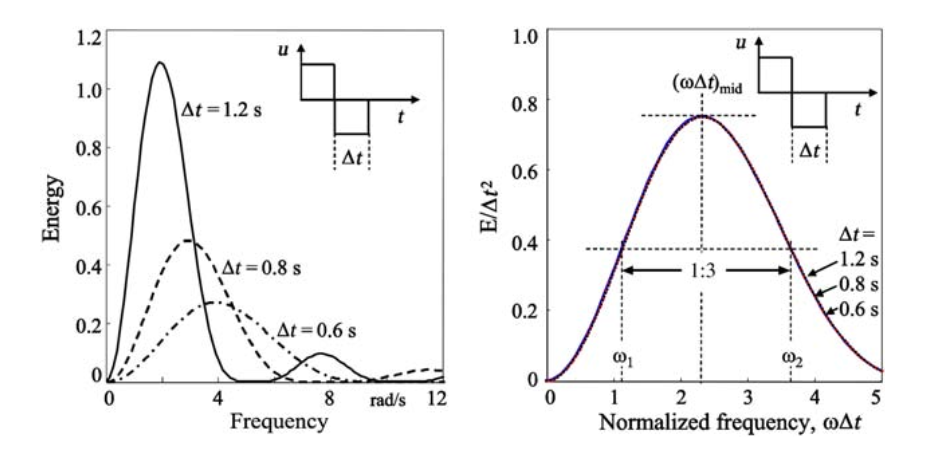
\includegraphics[width=\linewidth]{figuras/doblet}\\[0.2em]
      {\footnotesize \textit{Doublet} e seu espectro para diferentes $\Delta t$. Fonte: adaptado de Jategaonkar (2015)}
    \end{column}
    \begin{column}{0.5\textwidth}
      Sinal simétrico: energia nula em frequência zero e retorno ao \textit{hover}. O pico ocorre em $\omega_n\Delta t \approx 2{,}3$, o que dimensiona a manobra pela frequência do canal:
      \begin{equation*}
        \Delta t_{db} \approx \frac{2{,}3}{\omega_n} \approx \frac{T}{2{,}7} \tag{4.1}
      \end{equation*}
      Um \textit{doublet} por eixo: rolagem ($p$), arfagem ($q$) e guinada ($r$).
    \end{column}
  \end{columns}
\end{frame}

\begin{frame}{Critérios objetivos de uma boa manobra}
  Ruído de medição estimado do resíduo de alta frequência (filtro de Savitzky-Golay), robusto aos transitórios:
  \begin{align*}
    e_i &= \omega_i - \mathrm{SG}(\omega_i) \tag{4.2}\\
    \sigma_{\eta,i} &= 1{,}4826 \cdot \operatorname{med}\big|\,e_i - \operatorname{med}(e_i)\,\big| \tag{4.3}
  \end{align*}
  \begin{columns}[T]
    \begin{column}{0.5\textwidth}
      \textbf{Relação sinal-ruído} ($\geq 3$):
      \begin{equation*}
        \mathrm{SNR}_i = \frac{\sigma(\omega_i)}{\sigma_{\eta,i}} \tag{4.4}
      \end{equation*}
    \end{column}
    \begin{column}{0.5\textwidth}
      \textbf{Isolamento entre eixos} ($\rho_i \gg 1$):
      \begin{equation*}
        \rho_i = \frac{\sigma(\omega_i)}{\sqrt{\sum_{j\neq i}\sigma(\omega_j)^2}} \tag{4.5}
      \end{equation*}
    \end{column}
  \end{columns}
  \vspace{0.3em}
  {\footnotesize Também exigidos: faixa linear (sem saturar atuador), retorno ao \textit{trim} e repetibilidade.}
\end{frame}

\begin{frame}{Medições: aquisição e tratamento}
  \begin{center}
    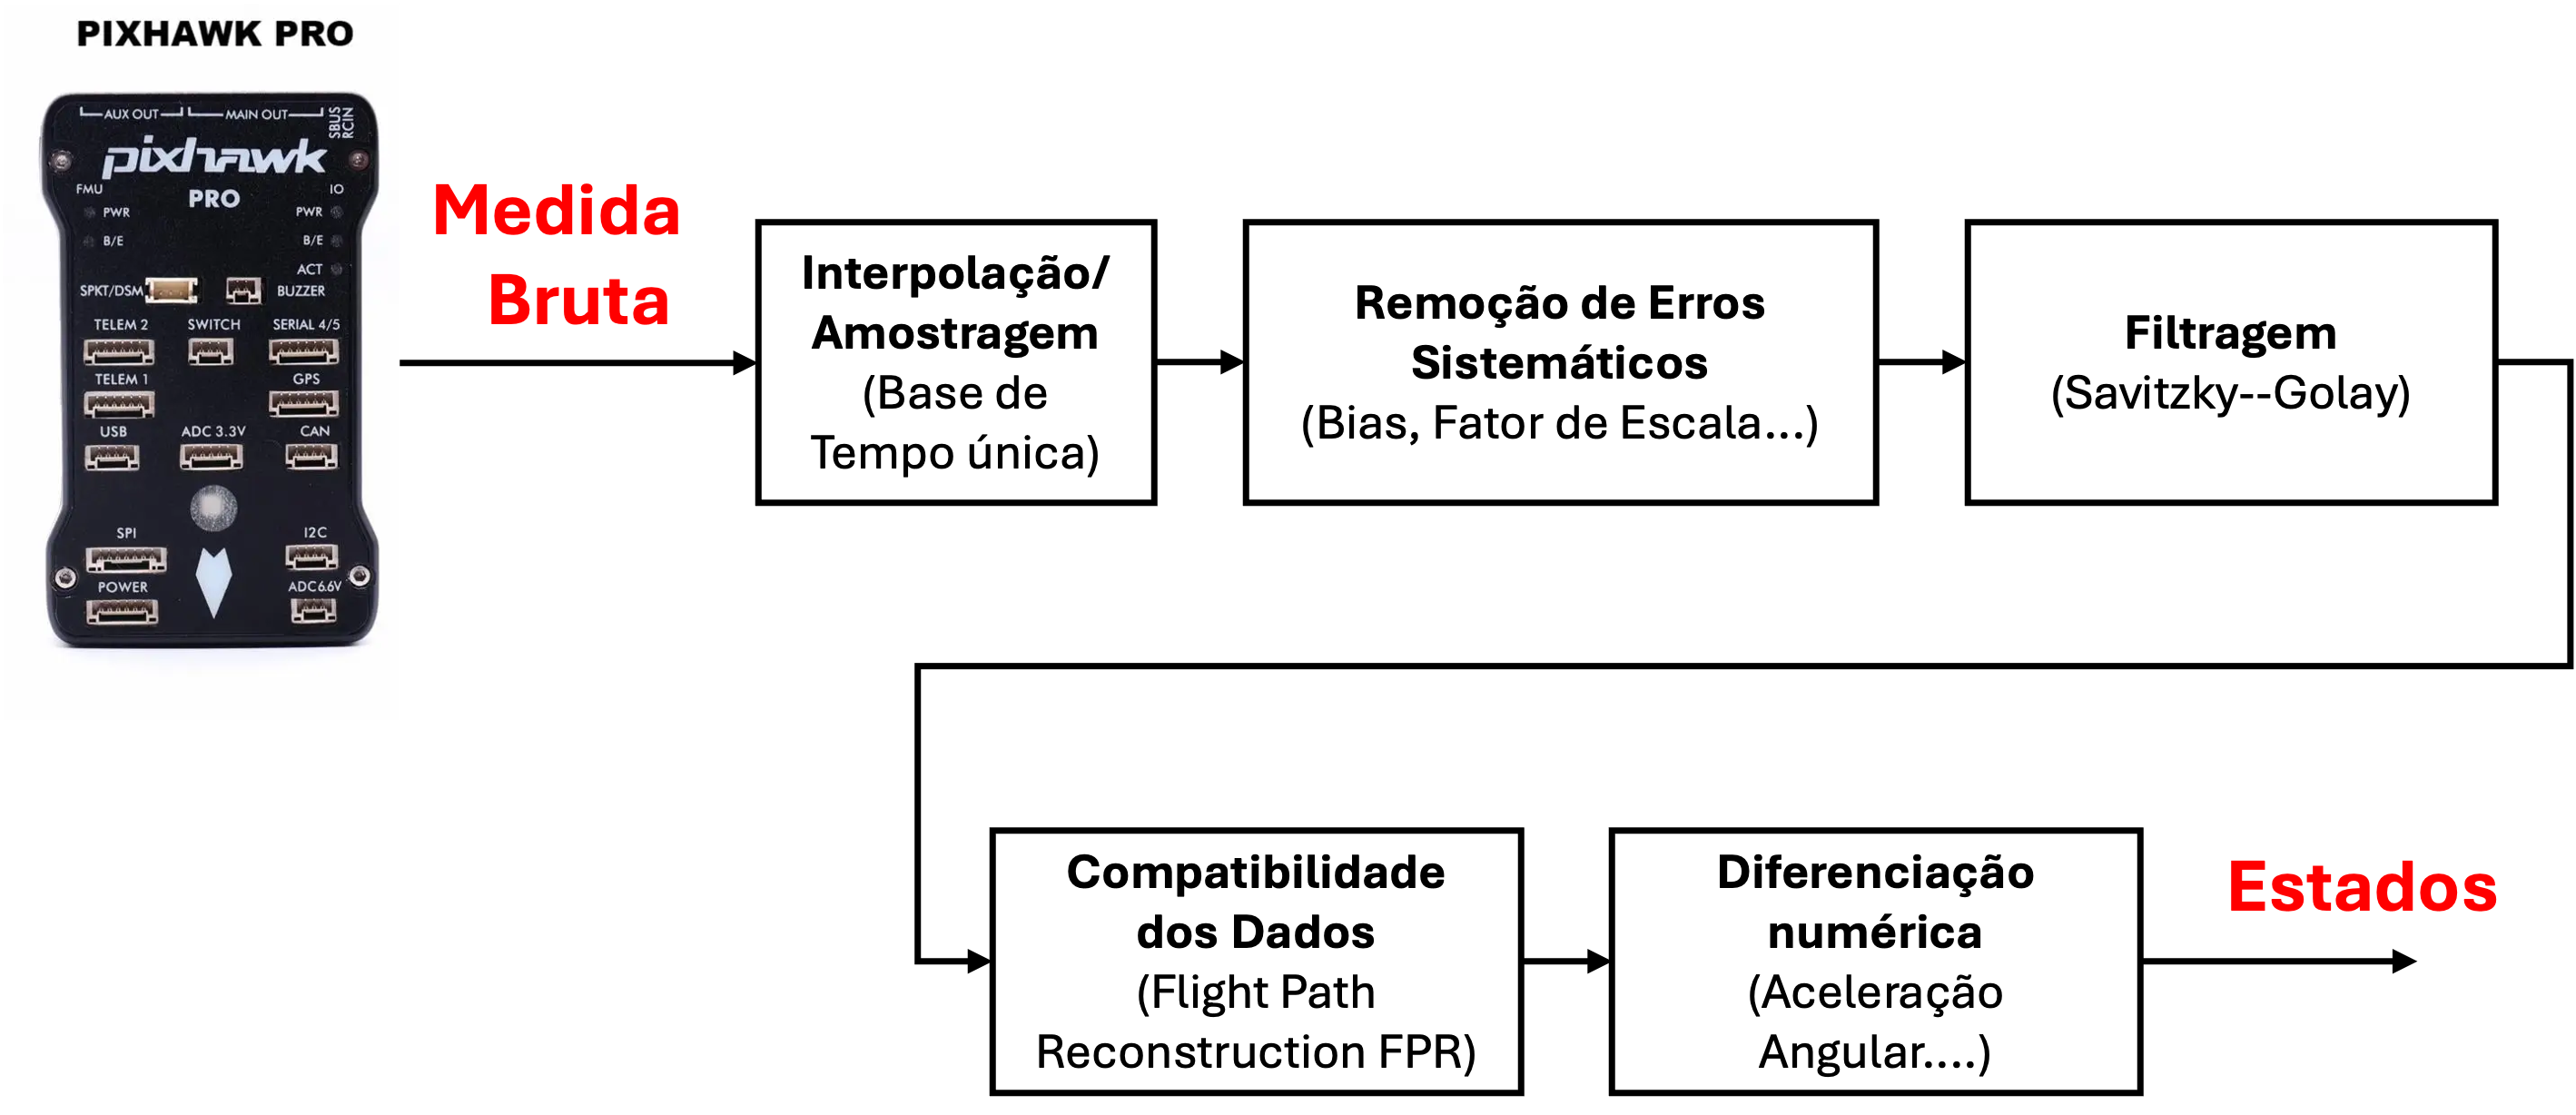
\includegraphics[width=0.7\linewidth]{figuras/measure}\\[0.2em]
    {\footnotesize Cadeia de aquisição: do log bruto ao vetor de medidas $z$ (Fig.~4.6)}
  \end{center}
  \begin{itemize}
    \item Taxa de amostragem comum de $10$~Hz (cerca de $5\times$ a banda do canal, abaixo de $2$~Hz), mesma ordem adotada por~\cite{Sato2021}.
    \item Correção de \textit{bias} do giroscópio e do acelerômetro em janelas calmas.
    \item Medidas: $p,q,r$ e $a_x,a_y,a_z$ (IMU), atitude $(\phi,\theta,\psi)$ do EKF e PWM $\sigma_{1\text{ a }4}$.
  \end{itemize}
\end{frame}

\begin{frame}{Métodos: EEM $+$ OEM}
  Dois métodos complementares no domínio do tempo~\cite{Jategaonkar2015}:
  \begin{itemize}
    \item \textbf{EEM} (erro de equação): estimativa inicial algébrica $\Theta_{\text{EEM}}$, ponderada por $\mathbf{W}_e$ nos 3 canais do resíduo $(\dot p,\dot q,\dot r)$.
    \item \textbf{OEM} (erro de saída): refino por máxima verossimilhança até $\Theta_{\text{OEM}}$, ponderado por $\mathbf{W}$ nos 6 canais de saída $(p,q,r,a_x,a_y,a_z)$.
  \end{itemize}
  A identificação foca na estimação do vetor de parâmetros:
  \begin{equation*}
    \Theta = [\,J_x,\,J_y,\,J_z,\,J_{xz},\;{c_T}_1,\dots,{c_T}_4,\;{c_M}_1,\dots,{c_M}_4,\;c_p,\,c_q,\,c_r\,]^\top \tag{4.8}
  \end{equation*}
\end{frame}

\begin{frame}{Processo de identificação em duas fases}
  \centering
  \resizebox{!}{6.15cm}{%
  \begin{tikzpicture}[
      node distance=0.6cm and 0.4cm,
      block/.style={rectangle, draw=blkEdge, semithick, rounded corners=2pt, fill=blkBase, text width=2.2cm, minimum height=0.7cm, align=center, font=\scriptsize},
      bigblock/.style={rectangle, draw=blkEdge, semithick, rounded corners=2pt, fill=blkBase, text width=2.8cm, minimum height=0.7cm, align=center, font=\scriptsize},
      smallblock/.style={rectangle, draw=blkEdge, semithick, rounded corners=2pt, fill=blkBase, text width=1.4cm, minimum height=0.55cm, align=center, font=\tiny},
      hi/.style={fill=blkHi, draw=blkHiEdge, thick},
      arrow/.style={-{Stealth[length=2mm]}, semithick, black!62},
      every node/.style={font=\scriptsize}
  ]
      \node[block, fill=blkBase, text width=3cm] (data) {Dados de Voo\\(PWM, $p,q,r$, $\phi,\theta,\psi$, IMU)};
      \node[block, below=0.5cm of data] (seg) {Segmentação Temporal};
      \node[smallblock, below left=0.5cm and 0.6cm of seg] (s1) {Seg. 1};
      \node[smallblock, below=0.5cm of seg] (s2) {Seg. 2};
      \node[smallblock, below right=0.5cm and 0.6cm of seg] (sn) {Seg. $N_s$};
      \node[smallblock, right=0.3cm of sn, fill=blkBase] (val) {Validação};
      \node[bigblock, below=1.2cm of s2, hi, text width=4cm] (eembox) {\textbf{Fase A: EEM}\\Concatena segmentos\\Estimação algébrica $\to \Theta_{\text{EEM}}$};
      \node[smallblock, left=0.9cm of eembox, text width=1.8cm] (theta0) {$\Theta_0$\\(valores iniciais)};
      \node[block, below=1.5cm of eembox, hi, xshift=-2.8cm, text width=2.3cm] (b1) {\textbf{Fase B.1} $\cdot$ OEM\\janela 1\,s\\$\Rightarrow \Theta_1$};
      \node[block, below=1.5cm of eembox, hi, text width=2.3cm] (b2) {\textbf{Fase B.2} $\cdot$ OEM\\janela 2\,s\\$\Rightarrow \Theta_2$};
      \node[block, below=1.5cm of eembox, hi, xshift=2.8cm, text width=2.3cm] (b3) {\textbf{Fase B.3} $\cdot$ OEM\\janela 3\,s\\$\Rightarrow \Theta_3$};
      \node[block, below=1.3cm of b2, hi, text width=3.0cm] (best) {Seleciona melhor $R^2$ na validação\\$\Rightarrow \Theta_{\text{OEM}}$};
      \draw[arrow] (data) -- (seg);
      \draw[arrow] (seg) -- (s1);
      \draw[arrow] (seg) -- (s2);
      \draw[arrow] (seg) -- (sn);
      \draw[arrow] (seg) -- (val);
      \draw[arrow] (s1) -- (eembox);
      \draw[arrow] (s2) -- (eembox);
      \draw[arrow] (sn) -- (eembox);
      \draw[arrow] (theta0) -- (eembox);
      \draw[arrow] (eembox.south) -- (b1.north);
      \draw[arrow] (eembox.south) -- node[pos=0.6, right, font=\tiny] {$\Theta_{\text{EEM}}$} (b2.north);
      \draw[arrow] (eembox.south) -- (b3.north);
      \draw[arrow] (b1.south) -- (best.north);
      \draw[arrow] (b2.south) -- (best.north);
      \draw[arrow] (b3.south) -- (best.north);
      \draw[arrow, dashed] (val.east) -- ++(1.4,0) |- (best.east);
  \end{tikzpicture}%
  }

  {\footnotesize O mesmo $\Theta_{\text{EEM}}$ alimenta em paralelo as três janelas da Fase B; retém-se o melhor $R^2$.}
\end{frame}

\begin{frame}{Fase A: \textit{Equation Error Method} (EEM)}
  Dispensa a integração numérica: avalia a equação dinâmica sobre os estados medidos. Resíduo de equação (Eqs.~4.17 a 4.19, dinâmica de taxa):
  \begin{equation*}
    e_{\text{EEM}}(t_k) = \dot{\boldsymbol{\omega}}_{\text{med}}(t_k) - f_\omega\big(\boldsymbol{\omega}_{\text{med}}(t_k),\,\boldsymbol{\tau}(t_k),\,\Theta_0\big) \tag{4.9}
  \end{equation*}
  com $\boldsymbol{\omega}_{\text{med}} = [p,q,r]^\top_{\text{med}}$. Parâmetros por mínimos quadrados ponderados sobre os segmentos de treino:
  \begin{equation*}
    \Theta_{\text{EEM}} = \arg\min_{\Theta} \sum_{k} \big\| \mathbf{W}_e^{1/2}\, e_{\text{EEM}}(t_k) \big\|^2, \qquad \mathbf{W}_e = \mathrm{diag}(1/\sigma_i^2) \tag{4.10}
  \end{equation*}
  Rápido e robusto (linear nos ganhos), porém as derivadas medidas amplificam o ruído e introduzem viés: serve como \textbf{ponto de partida}.
\end{frame}

\begin{frame}{Fase B: \textit{Output Error Method} (OEM)}
  \begin{columns}[c]
    \begin{column}{0.56\textwidth}
      Compara a saída \textbf{integrada} (Runge-Kutta de 4ª ordem) com a medição. Máxima verossimilhança (ruído gaussiano, covariância $\mathbf{R}_\nu$):
      \begin{equation*}
        J(\Theta) = \tfrac{1}{2}\sum_{k=1}^{N} [z_k - y_k]^\top \mathbf{R}_\nu^{-1} [z_k - y_k] \tag{4.11}
      \end{equation*}
      Minimizado por Gauss-Newton, equações normais com a informação de Fisher $F$:
      \begin{equation*}
        \underbrace{\Big[\textstyle\sum_k S_k^\top \mathbf{R}_\nu^{-1} S_k\Big]}_{F}\,\delta = \sum_k S_k^\top \mathbf{R}_\nu^{-1}(z_k - y_k) \tag{4.13}
      \end{equation*}
    \end{column}
    \begin{column}{0.44\textwidth}\centering
      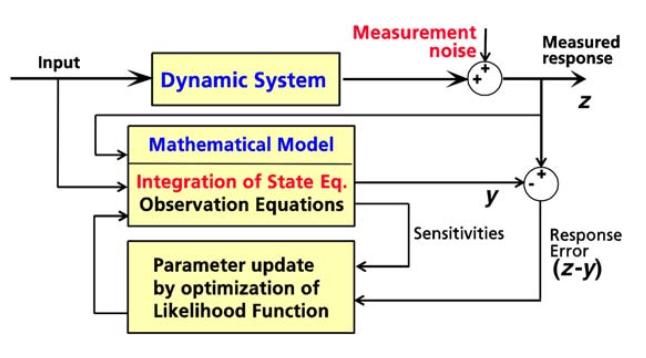
\includegraphics[width=0.82\linewidth]{figuras/oem_loop}\\[0.2em]
      {\footnotesize Ciclo iterativo do erro de saída. Fonte: adaptado de Jategaonkar (2015)}\\[0.3em]
      \begin{equation*}
        \Theta_{j+1} = \Theta_j + \delta \tag{4.14}
      \end{equation*}
      {\footnotesize $S = \partial y/\partial\Theta$ por diferenças finitas; $\mathbf{R}_\nu^{-1}\approx\mathbf{W}=\mathrm{diag}(1/\sigma_i^2)$; passo por \texttt{lsqnonlin} (\textit{trust-region}).}
    \end{column}
  \end{columns}
\end{frame}

\begin{frame}{Estratégia de multijanelas progressivas}
  A integração de um sistema instável pode divergir. Cada segmento de treino é dividido em janelas curtas e, no início de cada janela, o estado do modelo é \textbf{reinicializado com a medida}.
  \begin{itemize}
    \item Duração crescente $T_w = 1\,\text{s} \to 2\,\text{s} \to 3\,\text{s}$: as etapas curtas ajustam com baixo risco de divergência e as longas capturam a dinâmica mais lenta.
  \end{itemize}
  \begin{equation*}
    J(\Theta) = \sum_{s=1}^{N_s} \sum_{w} \sum_{k \in \mathcal{W}_w^{(s)}} \big\| \mathbf{W}^{1/2}[z_k - y_k]\big\|^2 \tag{4.15}
  \end{equation*}
  A cada estágio avalia-se o segmento de \textbf{validação} (fora da otimização) pelo $R^2$, retendo o melhor conjunto:
  \begin{equation*}
    R^2 = 1 - \frac{\sum_k (z_k - y_k)^2}{\sum_k (z_k - \bar{z})^2} \tag{4.16}
  \end{equation*}
\end{frame}

\begin{frame}{Modelos: forma de espaço de estados}
  Caixa cinza: a estrutura é fixada pelas leis de corpo rígido do Cap.~2 e apenas os parâmetros físicos são estimados.
  \begin{columns}[T]
    \begin{column}{0.5\textwidth}
      \begin{align*}
        \dot{\mathbf{x}}(t) &= f[\mathbf{x}(t),\mathbf{u}(t),\Theta] \tag{4.17}\\
        \mathbf{y}(t) &= g[\mathbf{x}(t),\mathbf{u}(t),\Theta] \tag{4.18}\\
        \mathbf{z}(t_k) &= \mathbf{y}(t_k) + \mathbf{v}(t_k) \tag{4.19}
      \end{align*}
      Saída observada (giroscópio $+$ acelerômetro):
      \begin{equation*}
        \mathbf{y} = [\,p,q,r,\,a_x,a_y,a_z\,]^\top \tag{4.21}
      \end{equation*}
    \end{column}
    \begin{column}{0.5\textwidth}
      \centering
      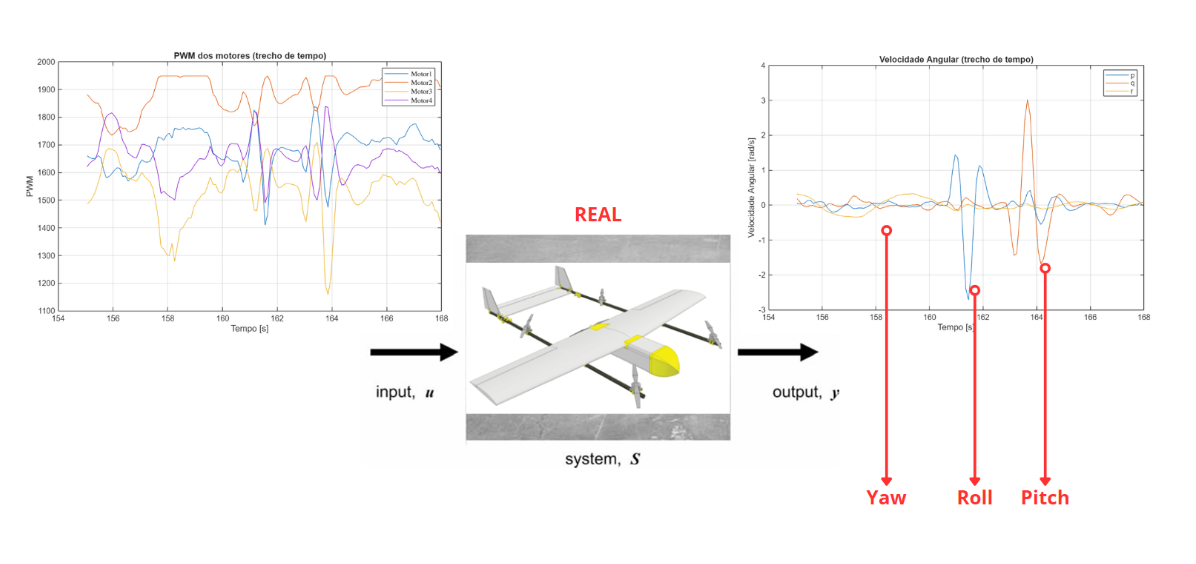
\includegraphics[width=\linewidth]{figuras/inout}\\[0.2em]
      {\footnotesize Modelo relacionando entradas e saídas medidas.}\par
      \vspace{0.7em}
      \raggedright\footnotesize As entradas $(T,\tau_x,\tau_y,\tau_z)$ são reconstruídas do PWM pelo modelo do motor e pela alocação: a própria entrada depende de $\Theta$ (os ${c_T}_i,{c_M}_i$).
    \end{column}
  \end{columns}
\end{frame}

\begin{frame}{Validação no domínio do tempo}
  Comparação com um segmento de \textbf{movimento composto}, fora da estimação. Quatro métricas complementares:
  \begin{columns}[T]
    \begin{column}{0.5\textwidth}
      \textbf{Coef. de determinação} $R^2$ (Eq.~4.16): aceitável acima de $0{,}5$.
      \vspace{0.4em}

      \textbf{Coef. de Theil} (TIC), bom se $\lesssim 0{,}25$:
      \begin{equation*}
        \mathrm{TIC} = \frac{\sqrt{\tfrac1N\sum_k(z_k-y_k)^2}}{\sqrt{\tfrac1N\sum_k z_k^2}+\sqrt{\tfrac1N\sum_k y_k^2}} \tag{4.22}
      \end{equation*}
    \end{column}
    \begin{column}{0.5\textwidth}
      \textbf{Decomposição de Theil} ($U^b+U^v+U^c=1$); ideal $U^c\approx 1$ (resíduo aleatório):
      \begin{equation*}
        U^{b}=\tfrac{(\bar z-\bar y)^2}{\mathrm{MSE}},\;
        U^{v}=\tfrac{(\sigma_z-\sigma_y)^2}{\mathrm{MSE}},\;
        U^{c}=\tfrac{2(1-\rho)\sigma_z\sigma_y}{\mathrm{MSE}} \tag{4.23}
      \end{equation*}
      \textbf{Cramér-Rao}: confiabilidade dos parâmetros; bem identificado se abaixo de $20\%$.
    \end{column}
  \end{columns}
\end{frame}

%=====================================================================
\section{Resultados e Validação}
%=====================================================================
\begin{frame}{Coerência dos dados de entrada}
  Antes de estimar, confronta-se a manobra planejada com a executada. A cadeia percorre todo o voo: piloto (RCIN) $\to$ PWM (RCOU) $\to$ momentos $(\tau_x,\tau_y,\tau_z)$ $\to$ taxas $(p,q,r)$.
  \begin{center}
    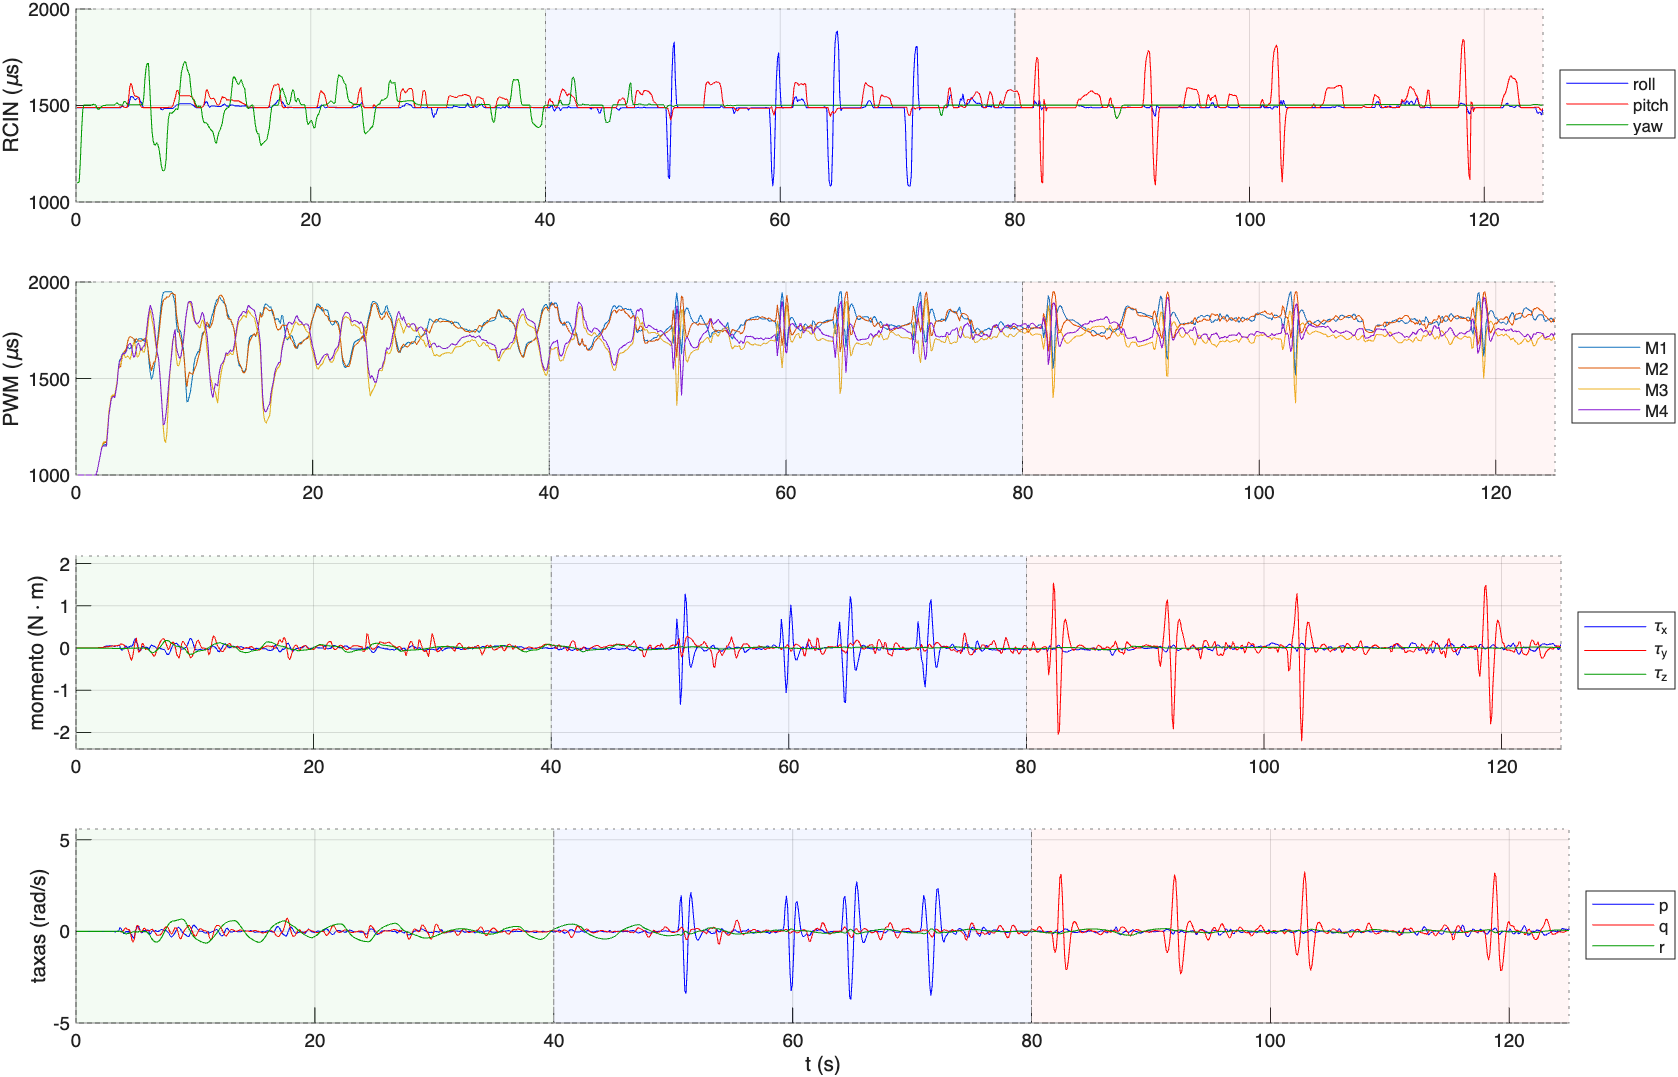
\includegraphics[width=0.5\linewidth]{figuras/excitacao_overview}\\[0.2em]
    {\footnotesize Cadeia de sinais da excitação ao longo do voo (Fig.~5.1)}
  \end{center}
\end{frame}

\begin{frame}{Critério de frequência: o \textit{doublet} por eixo}
  \begin{columns}[c]
    \begin{column}{0.56\textwidth}\centering
      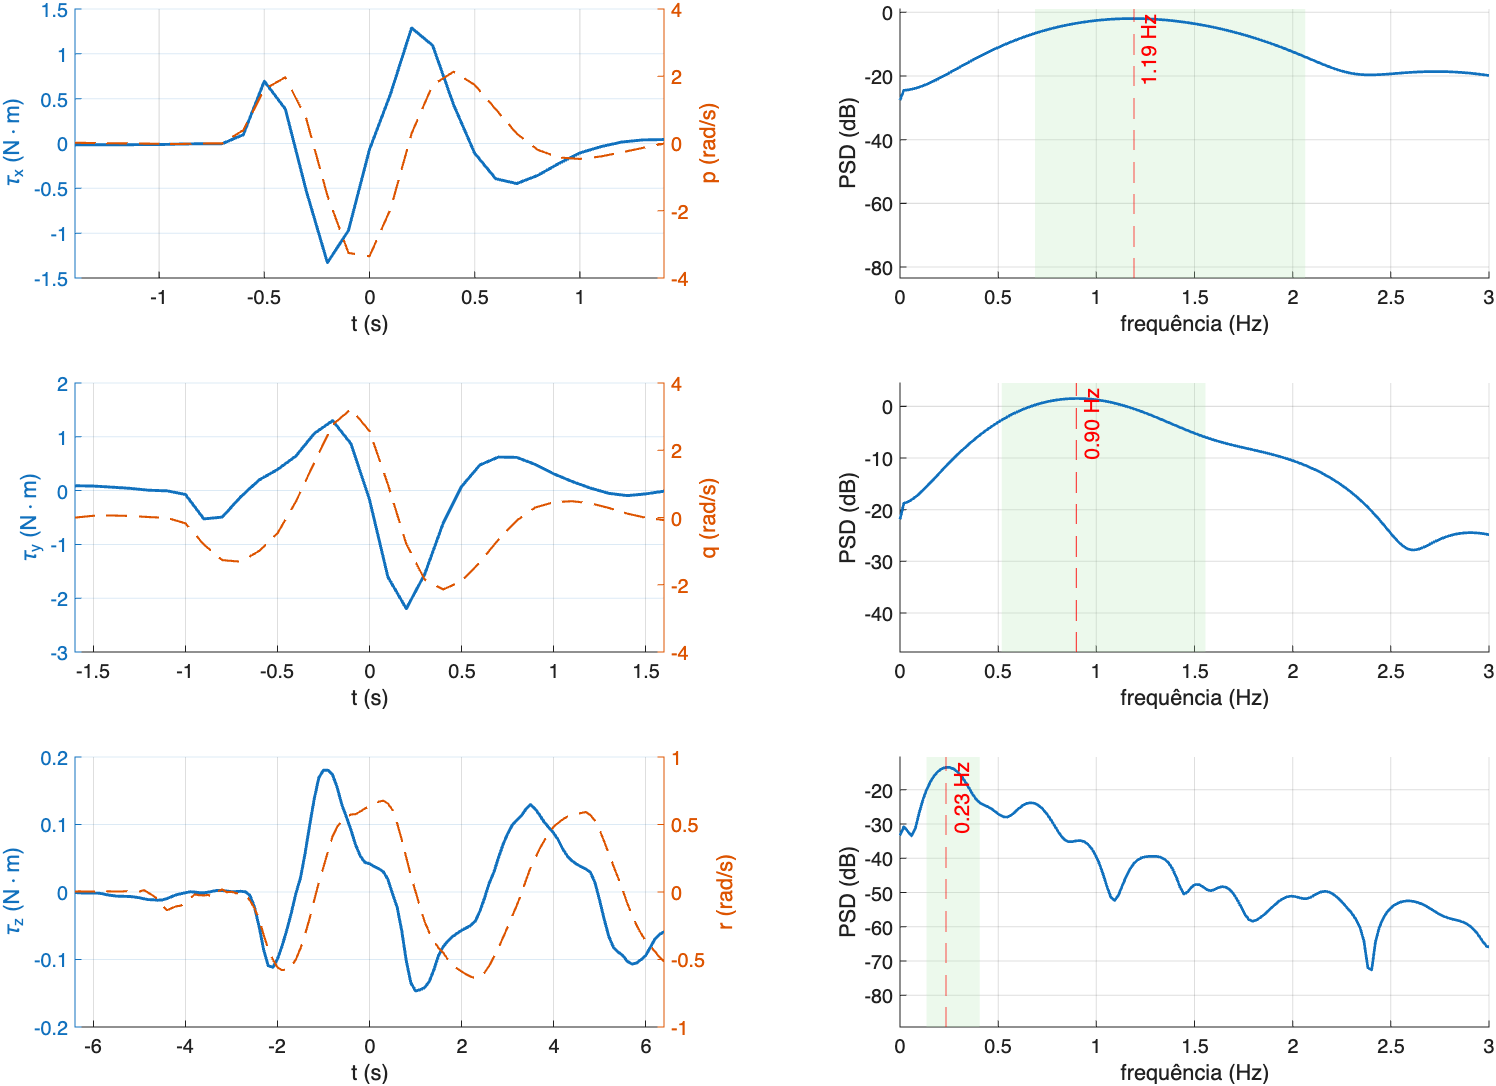
\includegraphics[width=\linewidth]{figuras/excitacao_doublet}\\[0.2em]
      {\footnotesize \textit{Doublet} no tempo e espectro, por eixo (Fig.~5.2)}
    \end{column}
    \begin{column}{0.44\textwidth}
      {\footnotesize
      \begin{tabular}{lccc}
        \toprule
        Eixo & $\sigma_\tau$ & $\Delta t$ & $f_{\text{pico}}$ \\
        \midrule
        Rolagem & 0,52 & 0,40 & 1,19 \\
        Arfagem & 0,71 & 0,40 & 0,90 \\
        Guinada & 0,07 & 2,00 & 0,23 \\
        \bottomrule
      \end{tabular}}

      {\scriptsize $\sigma_\tau$ [N$\cdot$m], $\Delta t$ [s], $f$ [Hz]}
      \vspace{0.5em}

      Rolagem e arfagem: \textit{doublet} nítido, energia $\approx 1$~Hz. \alert{Guinada}: cinco vezes mais lenta e fraca ($0{,}23$~Hz).
    \end{column}
  \end{columns}
\end{frame}

\begin{frame}{Relação sinal-ruído e isolamento}
  \begin{columns}[c]
    \begin{column}{0.58\textwidth}\centering
      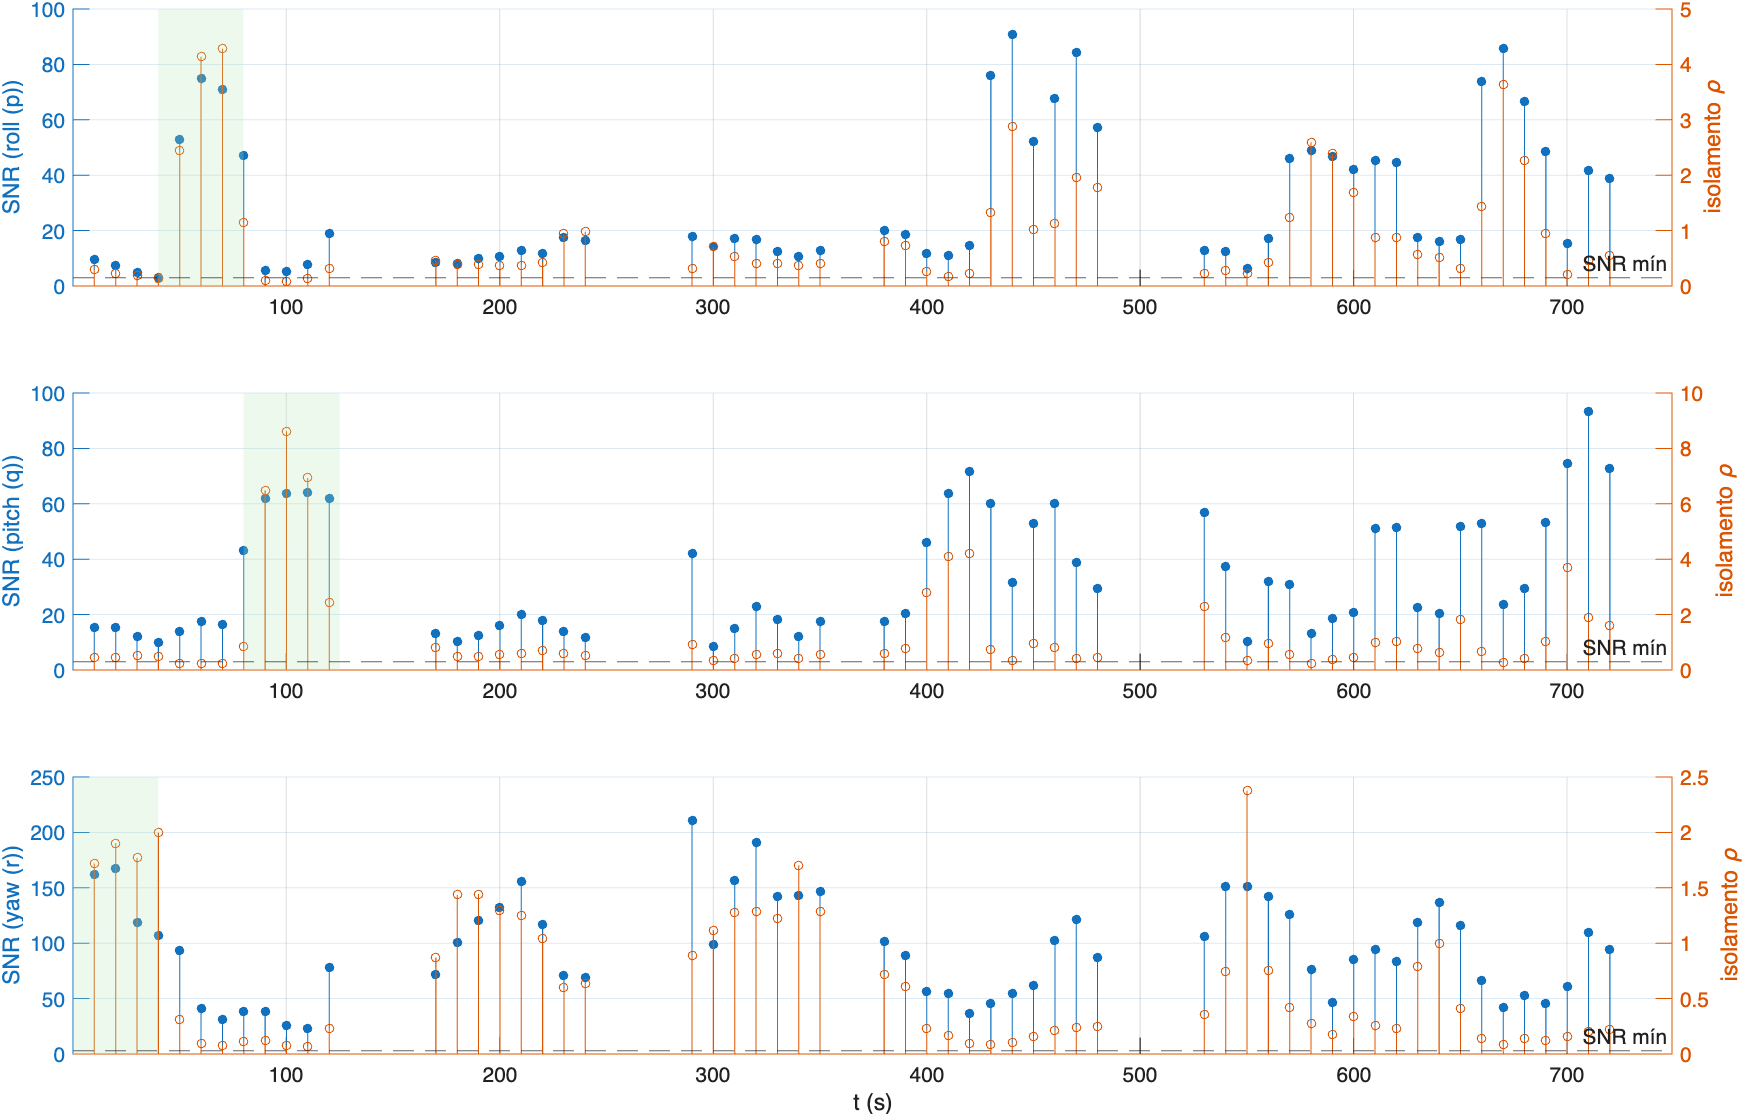
\includegraphics[width=\linewidth]{figuras/excitacao_snr}\\[0.2em]
      {\footnotesize SNR (azul) e isolamento $\rho$ (laranja) em janelas deslizantes (Fig.~5.3)}
    \end{column}
    \begin{column}{0.42\textwidth}
      {\footnotesize
      \begin{tabular}{lcc}
        \toprule
        Eixo & $\rho$ & SNR \\
        \midrule
        Rolagem & 3,2 & 62 \\
        Arfagem & 6,2 & 60 \\
        Guinada & 1,7 & 142 \\
        \bottomrule
      \end{tabular}}
      \vspace{0.5em}

      Todos superam SNR $\geq 3$. A \alert{guinada} tem o menor isolamento ($\rho=1{,}7$): $\tau_z$ vem só do contra-torque, cerca de $5\times$ menor.
    \end{column}
  \end{columns}
\end{frame}

\begin{frame}{Identificação: ponto de partida $\Theta_0$}
  Parte-se de $\Theta_0$ (inércias do CAD, motores de bancada, arrastos iniciais). O modelo inicial já reproduz a \emph{forma} da resposta, mas com erros de amplitude e amortecimento.
  \begin{center}
    
\includegraphics[width=0.5\linewidth]{figuras/id_sim_p0}\\[0.2em]
    {\footnotesize Resposta simulada de $\Theta_0$ frente às medições (Fig.~5.4)}
  \end{center}
\end{frame}

\begin{frame}{Parâmetros identificados e Cramér-Rao}
  \begin{columns}[c]
    \begin{column}{0.6\textwidth}\centering
      {\scriptsize
      \begin{tabular}{l cc cc}
        \toprule
        & \multicolumn{2}{c}{$\Theta_0$} & \multicolumn{2}{c}{$\Theta_{\text{OEM}}$} \\
        \cmidrule(lr){2-3}\cmidrule(lr){4-5}
        Parâm. & valor & CR\% & valor & CR\% \\
        \midrule
        $J_x$ & 0,0432 & 1,9 & 0,0469 & \textbf{1,8} \\
        $J_y$ & 0,0844 & 1,7 & 0,0984 & \textbf{1,7} \\
        $J_z$ & 0,1262 & 19,3 & 0,1453 & 19,2 \\
        $J_{xz}$ & 0,00157 & 70,3 & 0,00261 & \alert{30,4} \\
        $c_T$ (méd.) & 1,76 & 1,2 & 1,87 & \textbf{1,2} \\
        $c_M$ (méd.) & 5,04 & 48 & 3,48 & \alert{27} \\
        $c_p$ & 0,50 & 32,9 & 6,85 & \textbf{2,3} \\
        $c_q$ & 0,50 & 22,5 & 4,68 & \textbf{2,2} \\
        $c_r$ & 0,50 & 7,7 & 0,81 & \textbf{3,6} \\
        \bottomrule
      \end{tabular}}

      {\scriptsize $c_T$ em $10^{-7}$~N/RPM$^2$, $c_M$ em $10^{-9}$~N$\cdot$m/RPM$^2$ (Tab.~5.3)}
    \end{column}
    \begin{column}{0.4\textwidth}
      \begin{itemize}\footnotesize
        \item O OEM corrige o viés: $c_T\!\uparrow$, $c_M\!\downarrow\approx 30\%$, $J_x\!\uparrow 8{,}6\%$, $J_y\!\uparrow 16{,}6\%$.
        \item $J_x,J_y,c_T$ e arrastos: CR $<4\%$ (bem identificados).
        \item \alert{$c_M$ e $J_{xz}$} (guinada): CR $>20\%$, pior observabilidade.
      \end{itemize}
    \end{column}
  \end{columns}
\end{frame}

\begin{frame}{Melhora progressiva: $\Theta_0 \to$ EEM $\to$ OEM}
  \begin{columns}[c]
    \begin{column}{0.5\textwidth}\centering
      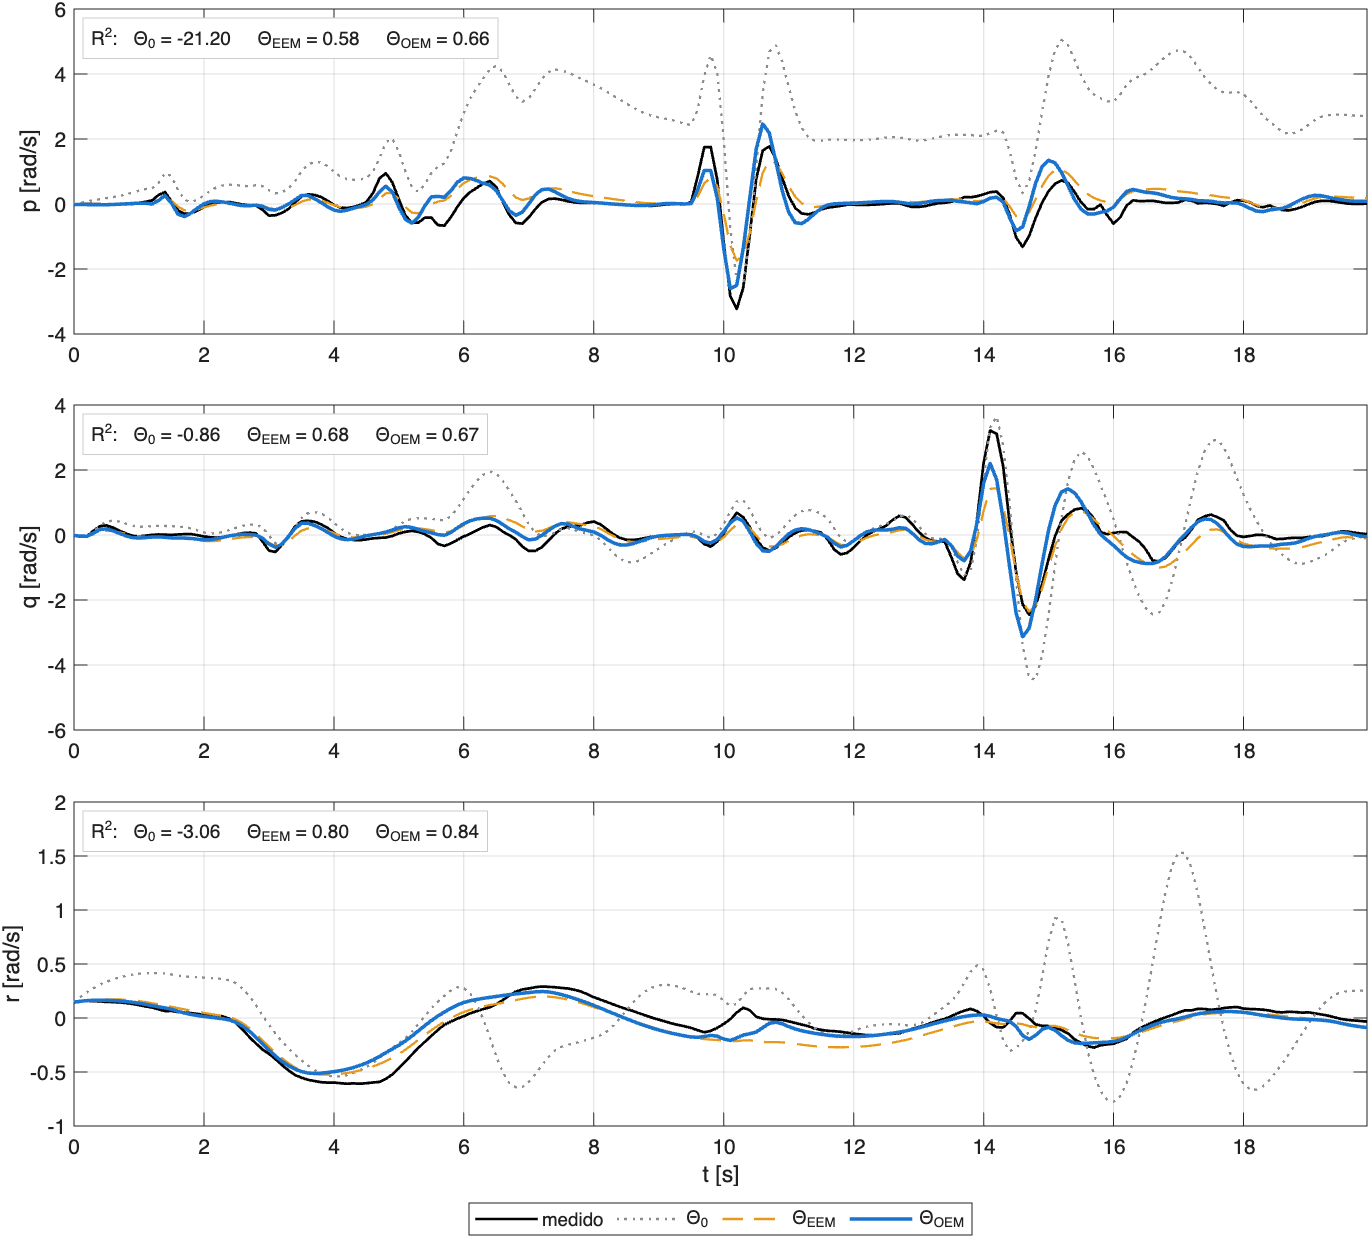
\includegraphics[width=0.8\linewidth]{figuras/id_comp_rates}\\[0.1em]
      {\footnotesize (a) Velocidades angulares}
    \end{column}
    \begin{column}{0.5\textwidth}\centering
      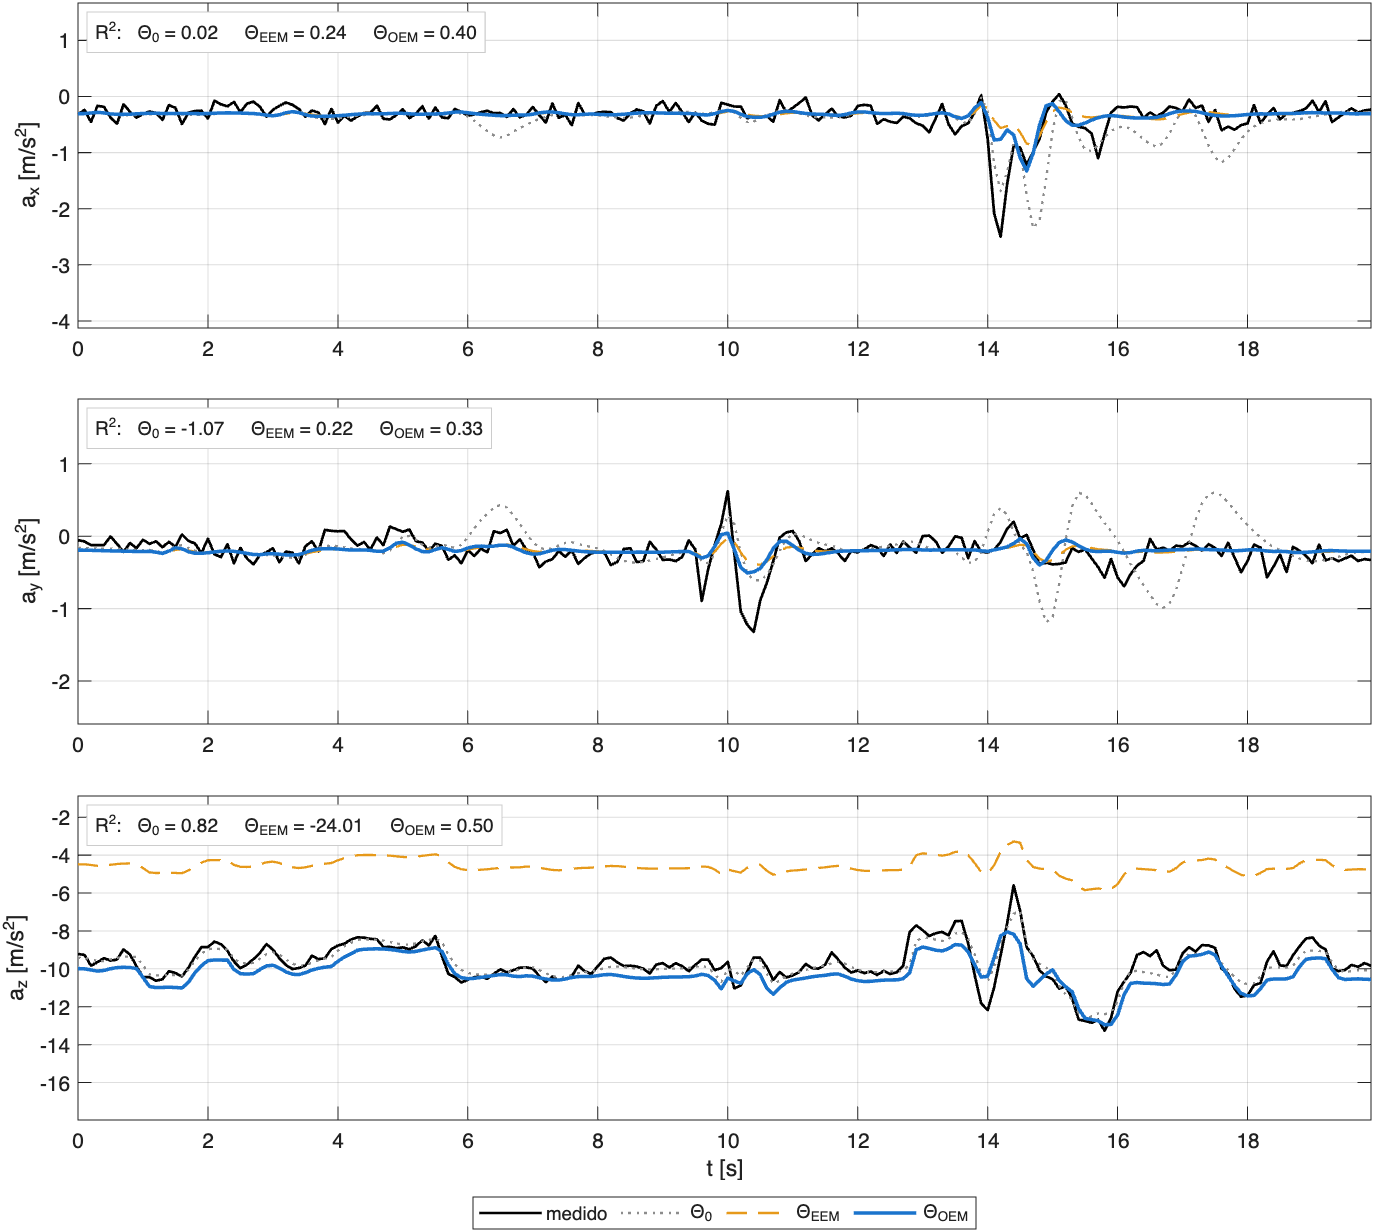
\includegraphics[width=0.8\linewidth]{figuras/id_comp_acc}\\[0.1em]
      {\footnotesize (b) Forças específicas}
    \end{column}
  \end{columns}
  \vspace{0.3em}
  {\footnotesize $\Theta_0$ diverge nas taxas (sobretudo em $p$); o EEM acompanha a forma; o OEM final adere às medições, com $R^2 = 0{,}66$, $0{,}67$ e $0{,}84$ em $p,q,r$ (Fig.~5.5).}
\end{frame}

\begin{frame}{Validação em segmento independente (605 a 625 s)}
  Segmento de movimento composto, fora da estimação. Comparação do modelo inicial $\Theta_0$ com o final (OEM):
  \begin{center}
  {\footnotesize
  \begin{tabular}{l ccc @{\hspace{1.6em}} ccc}
    \toprule
    & \multicolumn{3}{c}{$\Theta_0$ (inicial)} & \multicolumn{3}{c}{OEM (final)} \\
    \cmidrule(lr){2-4}\cmidrule(lr){5-7}
    Canal & $R^2$ & TIC & $U^c$ & $R^2$ & TIC & $U^c$ \\
    \midrule
    $p$   & \alert{$-21{,}2$} & 0,80 & 0,12 & 0,66 & 0,30 & 0,92 \\
    $q$   & $-0{,}86$ & 0,46 & 0,47 & 0,67 & 0,29 & 0,98 \\
    $r$   & $-3{,}06$ & 0,66 & 0,70 & 0,84 & 0,20 & 0,80 \\
    $a_x$ & 0,02 & 0,28 & 0,87 & 0,40 & 0,27 & 0,47 \\
    $a_y$ & $-1{,}07$ & 0,50 & 0,92 & 0,33 & 0,34 & 0,24 \\
    $a_z$ & 0,82 & 0,02 & 0,83 & 0,50 & 0,04 & 0,46 \\
    \bottomrule
  \end{tabular}}
  \end{center}
  \vfill
  {\footnotesize O $\Theta_0$ \alert{diverge} nas taxas ($R^2$ fortemente negativo, $-21{,}2$ em $p$): sem os parâmetros estimados, a integração foge das medidas. O \textbf{OEM} reproduz bem ($R^2$ até $0{,}84$), com o resíduo concentrado na \textbf{covariância} $U^c$ (0,80 a 0,98), erro essencialmente aleatório. Acelerômetro moderado, no limite do modelo de sensor. (Tabs.~5.4 e 5.5)}
\end{frame}

\begin{frame}{Projeto de controle: linearização e cascata}
  Sobre o modelo identificado, lineariza-se em torno do voo pairado (Taylor de 1ª ordem), $\delta\dot{\mathbf{x}} = \mathbf{A}\,\delta\mathbf{x} + \mathbf{B}\,\delta\mathbf{u}$ (Eq.~5.3), e projeta-se um controle em \textbf{cascata}~\cite{Hu2024, Idrissi2022, Mohsan2022} por alocação de polos.
  \begin{center}
    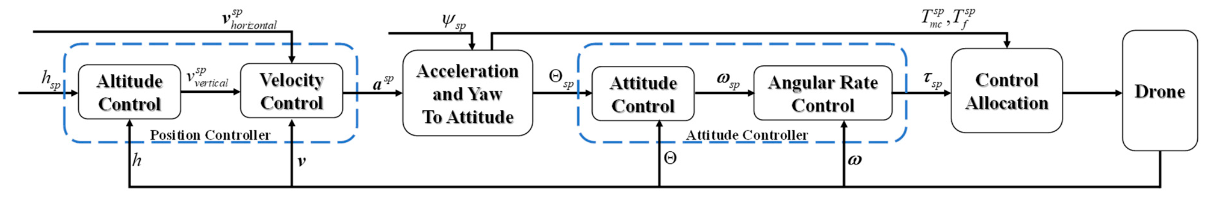
\includegraphics[width=\linewidth]{figuras/control}\\[0.2em]
    {\footnotesize Arquitetura PID em cascata: posição $\to$ atitude $\to$ alocação (Fig.~5.6)}
  \end{center}
  {\footnotesize A malha interna de velocidade angular é a própria dinâmica identificada por OEM: a qualidade da identificação propaga-se diretamente para os ganhos.}
\end{frame}

\begin{frame}{Malha fechada no modelo linear}
  \begin{columns}[c]
    \begin{column}{0.5\textwidth}\centering
      
\includegraphics[width=\linewidth]{figuras/sim_control_linear}
    \end{column}
    \begin{column}{0.5\textwidth}
      \begin{itemize}\footnotesize
        \item Degraus desacoplados: altitude $2$~m, avanço $3$~m/s, guinada $30^\circ$.
        \item Seguimento com erro de regime aproximadamente $0$; rolagem máxima de apenas $1{,}3^\circ$ (eixos desacoplados).
      \end{itemize}
      {\footnotesize Controle em cascata sobre o modelo linear, com saturação (Fig.~5.7).}
    \end{column}
  \end{columns}
\end{frame}

\begin{frame}{Controle: modelo linear vs não-linear}
  Aplica-se o \emph{mesmo} controlador às duas plantas. Duas não-linearidades, desprezadas na linearização, ganham peso longe do \textit{hover}:
  \begin{itemize}\footnotesize
    \item \textbf{acoplamento giroscópico} $-\Gamma_2\,q\,r$: gera rolagem quando $q$ e $r$ coexistem;
    \item \textbf{inclinação do empuxo}: ao arfar $\theta$, a componente vertical cai com $\cos\theta$ e a altitude afunda.
  \end{itemize}
  \begin{center}
  {\footnotesize
  \begin{tabular}{l ccc}
    \toprule
    Cenário & máx$|\Delta h|$ [m] & máx$|\Delta u|$ [m/s] & máx$|\Delta\phi|$ [$^\circ$] \\
    \midrule
    $S_1$ (suave) & 0,15 & 0,10 & 0,9 \\
    $S_2$ (média) & 0,56 & 1,08 & 3,9 \\
    $S_3$ (forte) & 1,55 & 11,1 & 17,9 \\
    \bottomrule
  \end{tabular}}\\[0.2em]
  {\footnotesize Desvio máximo entre as plantas nos três níveis (Tab.~5.10).}
  \end{center}
\end{frame}

\begin{frame}{Faixa de validade da linearização}
  \begin{columns}[T]
    \begin{column}{0.33\textwidth}\centering
      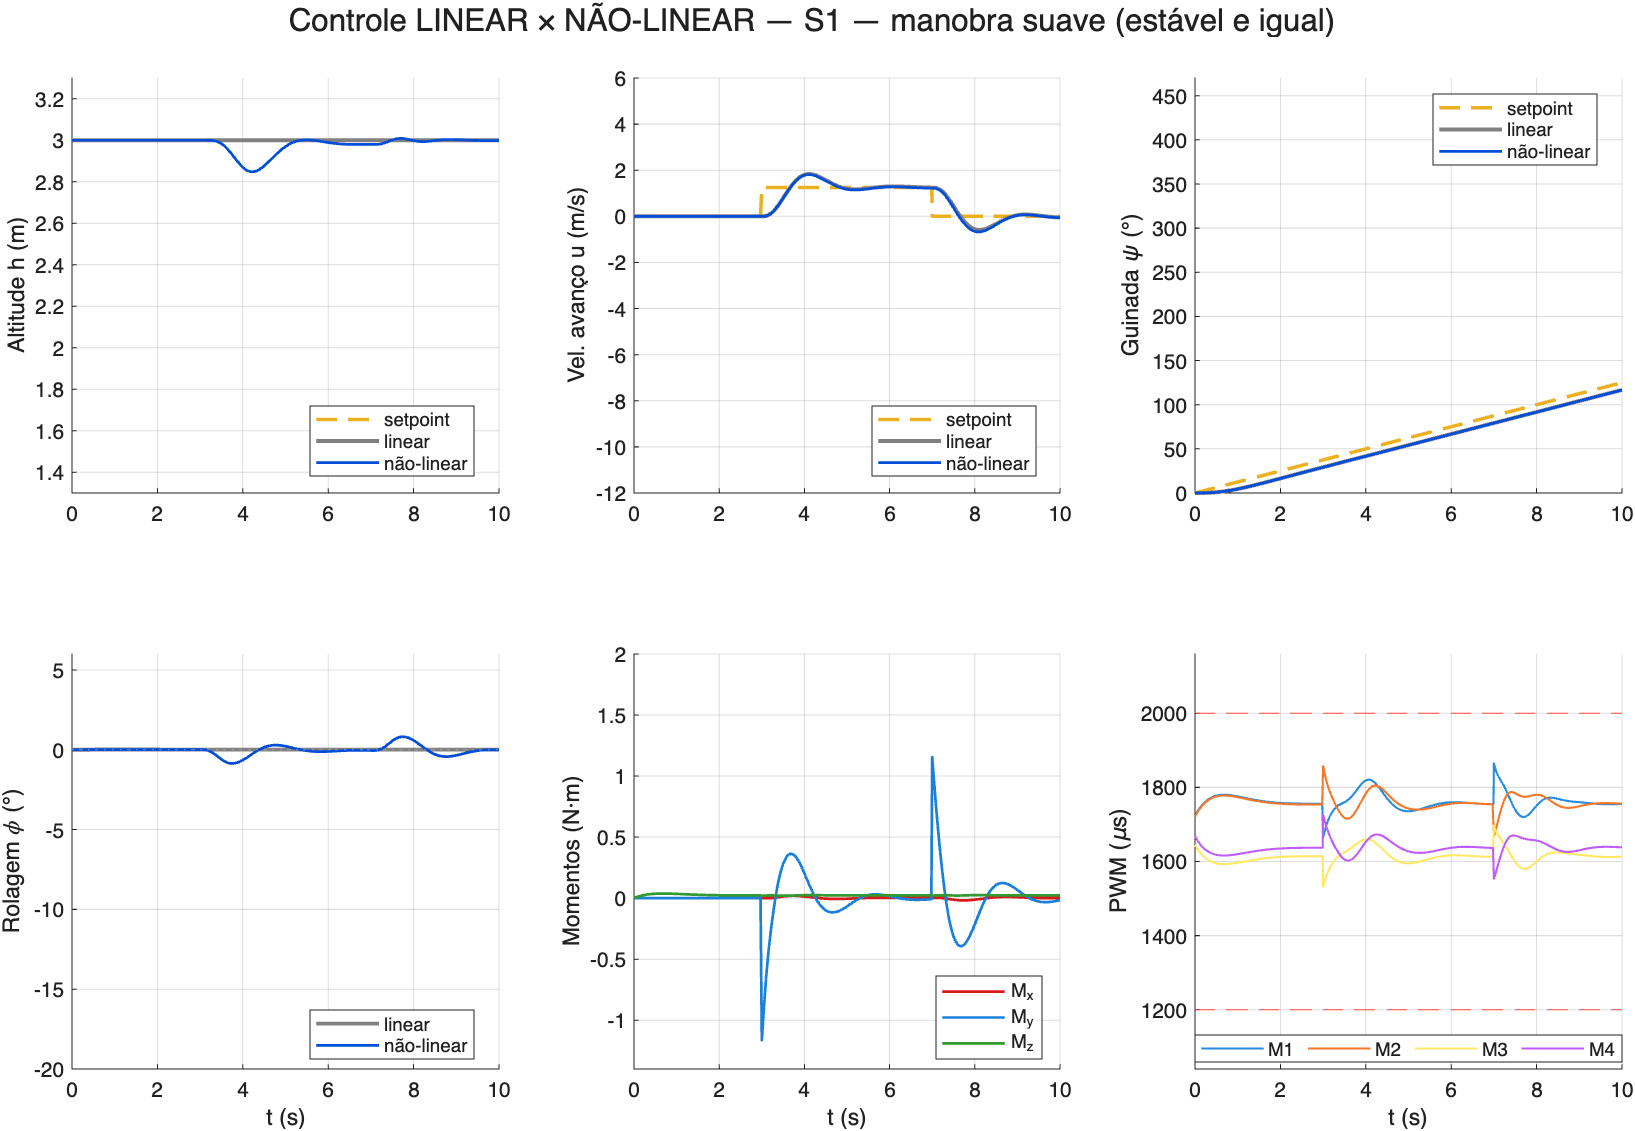
\includegraphics[width=\linewidth]{figuras/sim_ctrl_s1_igual}\\[0.1em]
      {\scriptsize $S_1$ suave: plantas \textbf{coincidem}}
    \end{column}
    \begin{column}{0.33\textwidth}\centering
      
\includegraphics[width=\linewidth]{figuras/sim_ctrl_s2_pouco}\\[0.1em]
      {\scriptsize $S_2$ média: divergência \textbf{pequena}}
    \end{column}
    \begin{column}{0.33\textwidth}\centering
      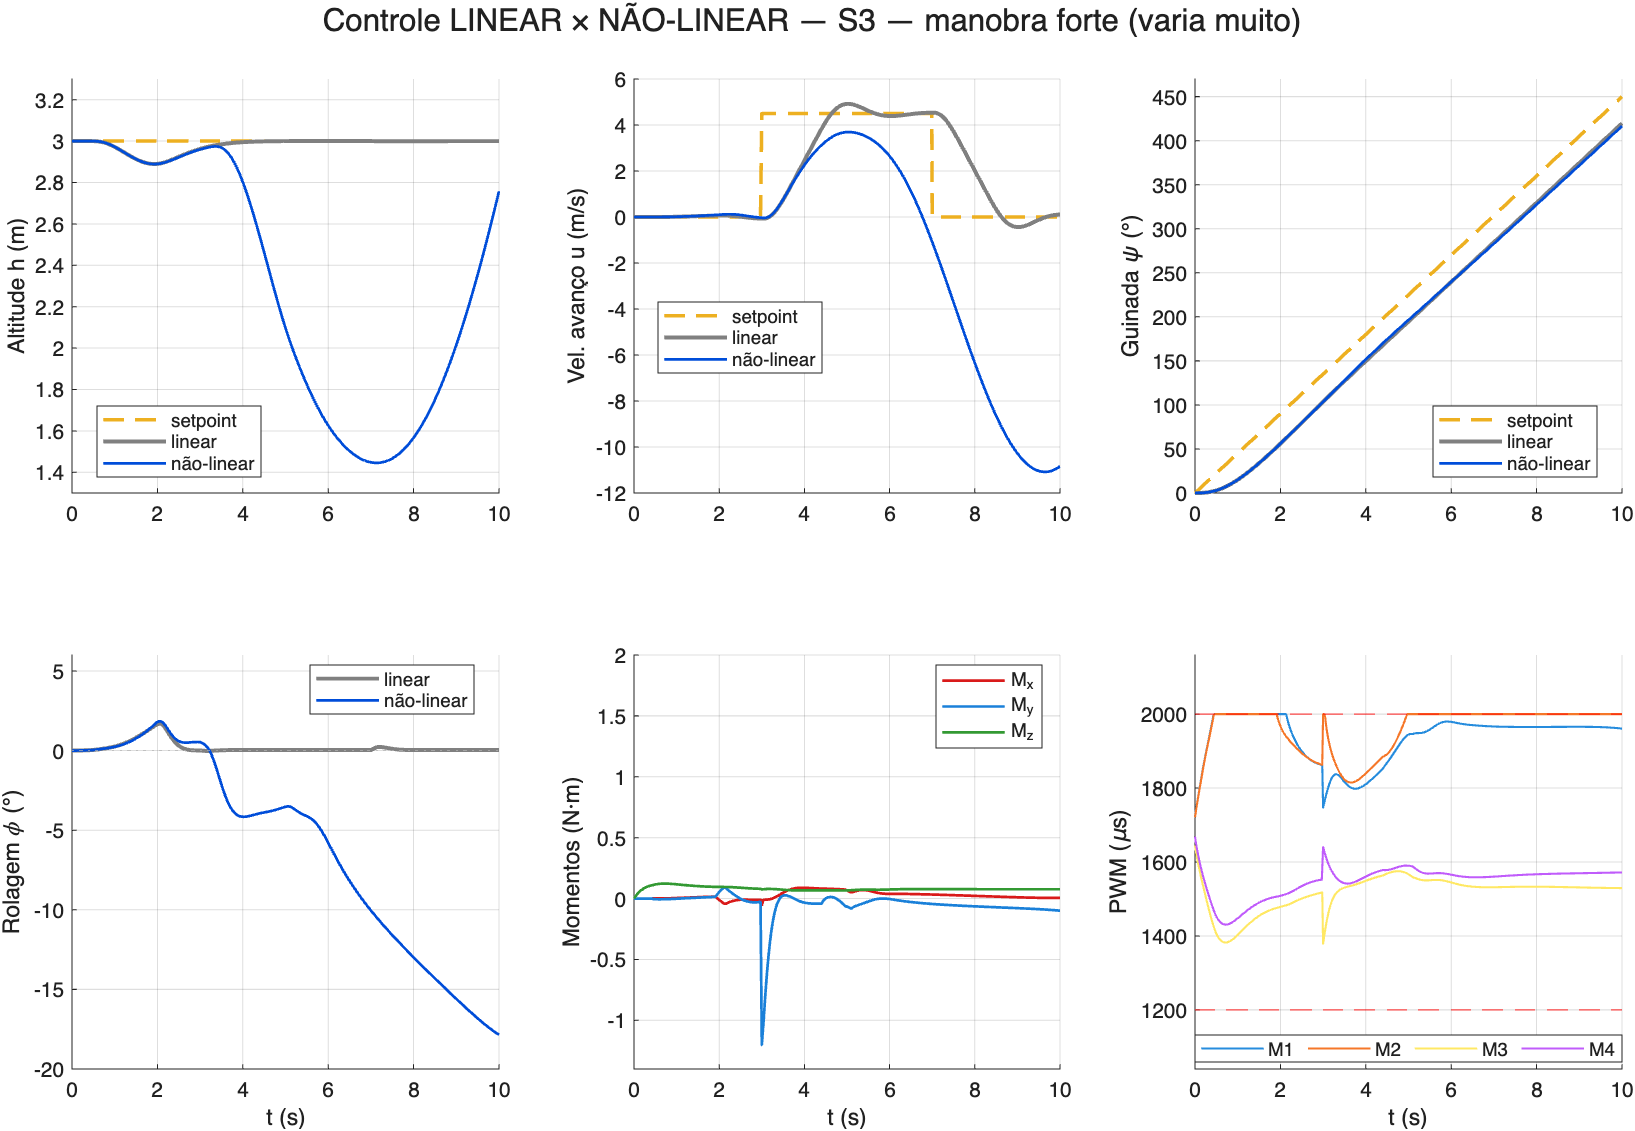
\includegraphics[width=\linewidth]{figuras/sim_ctrl_s3_muito}\\[0.1em]
      {\scriptsize $S_3$ forte: plantas \textbf{descolam}}
    \end{column}
  \end{columns}
  \vspace{0.3em}
  \begin{itemize}\footnotesize
    \item $S_1$: dentro do envelope do \textit{hover}, o linear reproduz fielmente a planta real.
    \item $S_3$: o não-linear afunda mais de $1{,}5$~m e a rolagem vai a $-18^\circ$ (giroscópico), enquanto o linear prevê resposta estável.
  \end{itemize}
  {\scriptsize Cinza: modelo linear. Azul: não-linear. Tracejado: \textit{setpoints} (Figs.~5.8 a 5.10).}
\end{frame}

%=====================================================================
\section{Conclusões}
%=====================================================================
\begin{frame}{Conclusões}
  \begin{itemize}
    \item Identificou-se um modelo não-linear do VTOL híbrido em modo multirrotor pela metodologia \textbf{M4V} (EEM inicial e OEM refinado), a partir de dados reais de voo.
    \item O modelo inicial $\Theta_0$ (CAD e bancada), embora fisicamente consistente, \alert{não reproduz} a dinâmica medida ($R^2$ negativo, integração diverge): a identificação a partir de dados é \textbf{essencial} antes de projetar o controle.
    \item O modelo do OEM reproduz bem as taxas ($R^2$ de $0{,}66$ a $0{,}84$), com resíduo essencialmente aleatório (parcela de covariância dominante).
    \item Projetou-se um controle em cascata sobre o modelo linearizado; a comparação linear vs não-linear \textbf{delimitou a faixa de validade} da linearização.
    \item Entrega-se uma \textbf{ferramenta de simulação} realista, banco de provas para o projeto e a sintonia de controladores antes do voo real.
  \end{itemize}
\end{frame}

\begin{frame}{Trabalhos futuros}
  \begin{itemize}
    \item \textbf{Modo híbrido}: acrescentar a aerodinâmica da asa (transição multirrotor para asa fixa) sobre a base confiável já validada.
    \item \textbf{Controle}: leis não-lineares ou robustas, com compensação direta dos termos de acoplamento.
    \item \textbf{Canal de guinada} (o mais fraco): manobras de excitação dedicadas e motores com maior contra-torque e empuxo para não perder altitude.
    \item \textbf{Instrumentação}: maior taxa de amostragem da IMU e estimação dos erros sistemáticos do acelerômetro e giroscópio como parâmetro do próprio OEM.
    \item \textbf{Estimação em tempo real}: observador acoplado ao controlador durante a campanha de voo.
  \end{itemize}
\end{frame}

%=====================================================================
\begin{frame}[allowframebreaks]{Referências}
  \setbeamertemplate{bibliography item}[text]
  \footnotesize
  \begin{thebibliography}{9}
    \bibitem{Shakhatreh2019} H.~Shakhatreh \textit{et al.}, ``Unmanned Aerial Vehicles (UAVs): A Survey on Civil Applications and Key Research Challenges,'' \textit{IEEE Access}, vol.~7, pp.~48572--48634, 2019.
    \bibitem{Hassanalian2017} M.~Hassanalian and A.~Abdelkefi, ``Classifications, applications, and design challenges of drones: A review,'' \textit{Progress in Aerospace Sciences}, vol.~91, pp.~99--131, 2017.
    \bibitem{Brito2019} R.~C.~Brito \textit{et al.}, ``A Comparative Approach on the use of UAVs Fixed-Wing and Rotative-Wing Applied to Precision Agriculture,'' in \textit{IEEE COMPSAC}, 2019, pp.~522--526.
    \bibitem{Saeed2018} A.~S.~Saeed, A.~B.~Younes, C.~Cai, and G.~Cai, ``A survey of hybrid Unmanned Aerial Vehicles,'' \textit{Progress in Aerospace Sciences}, vol.~98, pp.~91--105, 2018.
    \bibitem{Graesdal2021} B.~P.~Græsdal, ``Full Nonlinear System Identification for a Vertical-Takeoff-and-Landing UAV,'' M.Sc. thesis, NTNU, 2021.
    \bibitem{Bouabdallah2007} S.~Bouabdallah and R.~Siegwart, ``Full Control of a Quadrotor,'' in \textit{IEEE/RSJ IROS}, 2007, pp.~153--158.
    \bibitem{Carino2015} J.~Cariño Escobar, H.~Abaunza, and P.~Castillo, ``Quadrotor Quaternion Control,'' in \textit{ICUAS}, 2015, pp.~825--831.
    \bibitem{Aguirre2015} L.~A.~Aguirre, \textit{Introdução à Identificação de Sistemas}. Editora UFMG, 2015.
    \bibitem{Jategaonkar2015} R.~V.~Jategaonkar, \textit{Flight Vehicle System Identification: A Time-Domain Methodology}. AIAA, 2015.
    \bibitem{Beard2012} R.~W.~Beard and T.~W.~McLain, \textit{Small Unmanned Aircraft: Theory and Practice}. Princeton Univ. Press, 2012.
    \bibitem{Farrell2008} J.~A.~Farrell, \textit{Aided Navigation: GPS with High Rate Sensors}. McGraw-Hill, 2008.
    \bibitem{Quan2017} Q.~Quan, \textit{Introduction to Multicopter Design and Control}. Springer, 2017.
    \bibitem{Tischler2012} M.~B.~Tischler and R.~K.~Remple, \textit{Aircraft and Rotorcraft System Identification}, 2nd~ed. AIAA, 2012.
    \bibitem{DeLucena2025} A.~N.~de~Lucena, N.~M.~F.~de~Oliveira, F.~C.~Y.~C.~Sato, and L.~M.~G.~Gonçalves, ``Towards a rapidly manufactured VTOL hybrid UAV,'' in \textit{2025 Brazilian Conf. on Robotics (CROS)}, 2025.
    \bibitem{Matt2025} J.~J.~Matt, H.~Chao, M.~H.~Shawon, B.~C.~Svoboda, and S.~G.~Hagerott, ``System Identification for Small Flying-Wing Unmanned Aircraft Using Open-Loop and Closed-Loop Flight Data,'' \textit{Journal of Aircraft}, vol.~62, no.~4, 2025.
    \bibitem{Niermeyer2015} P.~Niermeyer, T.~Raffler, and F.~Holzapfel, ``Open-Loop Quadrotor Flight Dynamics Identification in Frequency Domain via Closed-Loop Flight Testing,'' in \textit{AIAA Guidance, Navigation, and Control Conf.}, 2015.
    \bibitem{Sato2021} F.~C.~Y.~C.~Sato, ``Identificação do Modelo Longitudinal do Aeromodelo Piper J3 pelo Método OEM,'' Dissertação (Mestrado), Instituto Tecnológico de Aeronáutica, São José dos Campos, 2021.
    \bibitem{Hu2024} J.~Hu, J.~Wei, K.~Liu, X.~Yu, M.~Cao, and Z.~Qin, ``Hybrid Mode: Routinization of the Transition Mode as the Third Common Mode for Compound VTOL Drones,'' \textit{Drones}, vol.~8, no.~3, p.~93, 2024.
    \bibitem{Idrissi2022} M.~Idrissi, M.~Salami, and F.~Annaz, ``A Review of Quadrotor Unmanned Aerial Vehicles: Applications, Architectural Design and Control Algorithms,'' \textit{J.~Intell. Robot. Syst.}, vol.~104, no.~2, p.~22, 2022.
    \bibitem{Mohsan2022} S.~A.~H.~Mohsan, M.~A.~Khan, F.~Noor, I.~Ullah, and M.~H.~Alsharif, ``Towards the Unmanned Aerial Vehicles (UAVs): A Comprehensive Review,'' \textit{Drones}, vol.~6, no.~6, p.~147, 2022.
    \bibitem{Bauersfeld2021} L.~Bauersfeld, E.~Kaufmann, P.~Foehn, S.~Sun, and D.~Scaramuzza, ``NeuroBEM: Hybrid Aerodynamic Quadrotor Model,'' in \textit{Robotics: Science and Systems (RSS)}, 2021.
    \bibitem{Cortez2022} H.~M.~M.~Cortez, ``Implementação de novas funcionalidades no sistema PixHawk,'' Dissertação (Mestrado), Instituto Tecnológico de Aeronáutica, São José dos Campos, 2022.
    \bibitem{Diorio2026} G.~Diório Cristofoletti, ``Bancada de caracterização dos motores do drone híbrido,'' in \textit{Anais do FIE}, 2026.
  \end{thebibliography}
\end{frame}

%=====================================================================
\begin{frame}[plain]
  \centering
  {\Huge \color{itaAzul} Obrigado!}\\[1em]
  {\large Perguntas?}\\[2em]
  \small Henrique Mark dos Santos Corrêa \\
  Orientadora: \orientadora
\end{frame}

\end{document}
